\documentclass[journal]{IEEEtran}
\usepackage{cite}
\usepackage{amsmath,amssymb,amsfonts}
\usepackage{algorithmic}
\usepackage{graphicx}
\usepackage{textcomp}
\usepackage{xcolor}
\usepackage{booktabs}
\usepackage{url}
\usepackage{array}
\usepackage{siunitx}
% AUTO-GENERATED by Paper/generate_paper_assets.py from results/final/*.json - do not edit by hand
\newcommand{\nRaw}{572}
\newcommand{\nRawPatients}{500}
\newcommand{\nClinical}{493}
\newcommand{\nClinicalPos}{305}
\newcommand{\nMatched}{347}
\newcommand{\nMatchedPos}{237}
\newcommand{\nTrain}{277}
\newcommand{\nTest}{70}
\newcommand{\nProteinSamples}{352}
\newcommand{\nProteinRaw}{487}
\newcommand{\nProteinKept}{456}
\newcommand{\nPCAll}{129}
\newcommand{\nEvents}{9}
\newcommand{\nEventsTrain}{8}
\newcommand{\nEventsTest}{1}
\newcommand{\nEventsAll}{12}
\newcommand{\nFeatFull}{18}
\newcommand{\nFeatPreop}{13}
\newcommand{\nSites}{9}
\newcommand{\nSiteTotal}{384}
\newcommand{\nExternal}{109}
\newcommand{\bpLOC}{0.775}
\newcommand{\bpFL}{0.790}
\newcommand{\bpFR}{0.782}
\newcommand{\bpCEN}{0.789}
\newcommand{\bpBL}{0.723}
\newcommand{\bpFLminusLOC}{+0.015\ [\ensuremath{-}0.007, +0.037]}
\newcommand{\bpFRminusFL}{\ensuremath{-}0.008\ [\ensuremath{-}0.013, \ensuremath{-}0.003]}
\newcommand{\bpCENminusFL}{\ensuremath{-}0.001\ [\ensuremath{-}0.004, +0.002]}
\newcommand{\bpFLminusBL}{+0.067\ [+0.048, +0.086]}
\newcommand{\bpLcPartOne}{0.696}
\newcommand{\bpLcFrOne}{0.751}
\newcommand{\bpLcPartAll}{0.838}
\newcommand{\bpLcFrAll}{0.785}
\newcommand{\bpLooShapRho}{0.48\ [0.34, 0.62]}
\newcommand{\bpShapSizeRho}{0.51}
\newcommand{\bpMacroSites}{7.4}
\newcommand{\cvFull}{0.818}
\newcommand{\cvPreop}{0.642}
\newcommand{\cvProt}{0.574}
\newcommand{\cvFullProt}{0.659}
\newcommand{\cvSkFull}{0.824}
\newcommand{\cvRFFullProt}{0.782}
\newcommand{\cvRFFull}{0.803}
\newcommand{\cvProtDiff}{\ensuremath{-}0.159\ [\ensuremath{-}0.188, \ensuremath{-}0.130]}
\newcommand{\cvPreopDiff}{+0.176\ [+0.148, +0.203]}
\newcommand{\cvProtPreopDiff}{\ensuremath{-}0.047\ [\ensuremath{-}0.080, \ensuremath{-}0.013]}
\newcommand{\nFolds}{25}
\newcommand{\driftRedMin}{32.0}
\newcommand{\driftRedMax}{36.4}
\newcommand{\driftAvgIID}{0.206}
\newcommand{\driftAvgSkew}{0.770}
\newcommand{\driftMuZero}{0.599}
\newcommand{\driftMuOne}{0.268}
\newcommand{\sigmaTen}{5.68}
\newcommand{\sigmaFive}{10.55}
\newcommand{\sigmaTwo}{24.99}
\newcommand{\sigmaOne}{49.02}
\newcommand{\sigmaHalf}{97.01}
\newcommand{\auNoDP}{0.823}
\newcommand{\auAvgTen}{0.821}
\newcommand{\auProxTen}{0.823}
\newcommand{\auLossTen}{\ensuremath{-}0.002\ [\ensuremath{-}0.009, +0.005]}
\newcommand{\auAvgFive}{0.818}
\newcommand{\auProxFive}{0.821}
\newcommand{\auLossFive}{\ensuremath{-}0.005\ [\ensuremath{-}0.014, +0.003]}
\newcommand{\auAvgTwo}{0.800}
\newcommand{\auProxTwo}{0.812}
\newcommand{\auLossTwo}{\ensuremath{-}0.023\ [\ensuremath{-}0.038, \ensuremath{-}0.008]}
\newcommand{\auAvgOne}{0.761}
\newcommand{\auProxOne}{0.789}
\newcommand{\auLossOne}{\ensuremath{-}0.063\ [\ensuremath{-}0.087, \ensuremath{-}0.038]}
\newcommand{\auAvgHalf}{0.691}
\newcommand{\auProxHalf}{0.720}
\newcommand{\auLossHalf}{\ensuremath{-}0.132\ [\ensuremath{-}0.180, \ensuremath{-}0.085]}
\newcommand{\gridSup}{12}
\newcommand{\gridCells}{20}
\newcommand{\gridSupCtl}{3}
\newcommand{\gridNoDPmax}{0.0019}
\newcommand{\gridOneHalfMin}{0.028}
\newcommand{\gridOneHalfMax}{0.030}
\newcommand{\gridCtlOneHalfMax}{0.003}
\newcommand{\pflLocalThree}{0.754}
\newcommand{\pflProxThree}{0.811}
\newcommand{\pflPFLThree}{0.805}
\newcommand{\pflGainThree}{+0.051\ [+0.015, +0.086]}
\newcommand{\pflVsProxThree}{\ensuremath{-}0.006\ [\ensuremath{-}0.022, +0.011]}
\newcommand{\pflLocalFive}{0.796}
\newcommand{\pflProxFive}{0.817}
\newcommand{\pflPFLFive}{0.814}
\newcommand{\pflGainFive}{+0.018\ [\ensuremath{-}0.021, +0.057]}
\newcommand{\pflVsProxFive}{\ensuremath{-}0.003\ [\ensuremath{-}0.011, +0.005]}
\newcommand{\pflLocalTen}{0.785}
\newcommand{\pflProxTen}{0.841}
\newcommand{\pflPFLTen}{0.838}
\newcommand{\pflGainTen}{+0.053\ [+0.010, +0.096]}
\newcommand{\pflVsProxTen}{\ensuremath{-}0.003\ [\ensuremath{-}0.014, +0.007]}
\newcommand{\shRhoTenThree}{0.68}
\newcommand{\shRhoHalfThree}{0.25}
\newcommand{\shTSTenThree}{0.79}
\newcommand{\shTSHalfThree}{0.51}
\newcommand{\shRRHalfThree}{0.57}
\newcommand{\shLooThree}{0.68\ [0.42, 0.93]}
\newcommand{\shSizeThree}{0.55\ [0.31, 0.79]}
\newcommand{\shRThree}{5}
\newcommand{\shRhoTenFive}{0.66}
\newcommand{\shRhoHalfFive}{0.30}
\newcommand{\shTSTenFive}{0.65}
\newcommand{\shTSHalfFive}{0.41}
\newcommand{\shRRHalfFive}{0.74}
\newcommand{\shLooFive}{0.34\ [0.14, 0.54]}
\newcommand{\shSizeFive}{0.33\ [0.11, 0.55]}
\newcommand{\shRFive}{5}
\newcommand{\shRhoTenTen}{0.73}
\newcommand{\shRhoHalfTen}{0.36}
\newcommand{\shTSTenTen}{0.62}
\newcommand{\shTSHalfTen}{0.30}
\newcommand{\shRRHalfTen}{0.88}
\newcommand{\shLooTen}{0.44\ [0.30, 0.58]}
\newcommand{\shSizeTen}{0.46\ [0.35, 0.58]}
\newcommand{\shRTen}{2}
\newcommand{\miaNoDP}{0.511\ [0.489, 0.533]}
\newcommand{\miaOne}{0.510\ [0.484, 0.537]}
\newcommand{\miaHalf}{0.512\ [0.490, 0.534]}
\newcommand{\miaCtl}{0.659\ [0.640, 0.678]}
\newcommand{\miaGap}{+0.017\ [\ensuremath{-}0.007, +0.041]}
\newcommand{\shiftCovTwo}{0.765}
\newcommand{\shiftConTwo}{0.498}
\newcommand{\shiftBase}{0.826}
\newcommand{\abCen}{0.823}
\newcommand{\abAvg}{0.824}
\newcommand{\abProx}{0.826}
\newcommand{\abDPFive}{0.820}
\newcommand{\abDPOne}{0.787}
\newcommand{\abPreop}{0.659}
\newcommand{\abProt}{0.682}
\newcommand{\pNineN}{5{,}610}
\newcommand{\pNinePos}{2{,}146}
\newcommand{\pNineHosp}{19}
\newcommand{\pNineCountries}{8}
\newcommand{\pNinePrevLo}{12}
\newcommand{\pNinePrevHi}{60}
\newcommand{\pNinePrev}{38.3}
\newcommand{\pNineReps}{50}
\newcommand{\pRepNohBL}{0.827}
\newcommand{\pRepNohLOC}{0.818}
\newcommand{\pRepNohCEN}{0.827}
\newcommand{\pRepNohFL}{0.826}
\newcommand{\pRepNohFR}{0.827}
\newcommand{\pRepEttBL}{0.792}
\newcommand{\pRepEttLOC}{0.799}
\newcommand{\pRepEttCEN}{0.813}
\newcommand{\pRepEttFL}{0.803}
\newcommand{\pRepEttFR}{0.803}
\newcommand{\pSLOC}{0.829}
\newcommand{\pWLOC}{0.857}
\newcommand{\pSFL}{0.824}
\newcommand{\pWFL}{0.856}
\newcommand{\pSProx}{0.821}
\newcommand{\pWProx}{0.853}
\newcommand{\pSCEN}{0.825}
\newcommand{\pWCEN}{0.856}
\newcommand{\pSFR}{0.822}
\newcommand{\pWFR}{0.854}
\newcommand{\pSNoh}{0.834}
\newcommand{\pWNoh}{0.850}
\newcommand{\pSEtt}{0.795}
\newcommand{\pWEtt}{0.832}
\newcommand{\pDFLminusLOC}{\ensuremath{-}0.005\ [\ensuremath{-}0.015, +0.006]}
\newcommand{\pDFRminusFL}{\ensuremath{-}0.002\ [\ensuremath{-}0.002, \ensuremath{-}0.001]}
\newcommand{\pDCENminusFL}{+0.002\ [\ensuremath{-}0.001, +0.004]}
\newcommand{\pDFLminusNoh}{\ensuremath{-}0.010\ [\ensuremath{-}0.016, \ensuremath{-}0.005]}
\newcommand{\pDFLminusEtt}{+0.029\ [+0.023, +0.035]}
\newcommand{\pDProxminusFL}{\ensuremath{-}0.003\ [\ensuremath{-}0.005, \ensuremath{-}0.000]}
\newcommand{\pGainSig}{4}
\newcommand{\pLossSig}{4}
\newcommand{\pGainSizeRho}{\ensuremath{-}0.26}
\newcommand{\pLcFrOne}{0.769}
\newcommand{\pLcFrFive}{0.815}
\newcommand{\pLcFrLast}{0.830}
\newcommand{\pFrOE}{0.99}
\newcommand{\pFrSlope}{1.03}
\newcommand{\pDriftRed}{30.8}
\newcommand{\pDpLossHalf}{\ensuremath{-}0.005\ [\ensuremath{-}0.011, +0.001]}
\newcommand{\pDpLossOne}{\ensuremath{-}0.004\ [\ensuremath{-}0.008, +0.001]}
\newcommand{\pDpLossFive}{\ensuremath{-}0.002\ [\ensuremath{-}0.007, +0.003]}
\newcommand{\pProxHalfMax}{0.001}
\newcommand{\pSigmaHalf}{97}
\newcommand{\pPflSmall}{+0.039\ [+0.013, +0.065]}
\newcommand{\pPflAll}{+0.010\ [+0.005, +0.016]}
\newcommand{\pPflLarge}{+0.001\ [+0.000, +0.001]}
\newcommand{\pPflLargeLoc}{\ensuremath{-}0.005\ [\ensuremath{-}0.007, \ensuremath{-}0.004]}
\newcommand{\pNSmall}{4}
\newcommand{\pMiaNoDP}{0.500}
\newcommand{\pMiaCtl}{0.937}
\newcommand{\pLocoAvgNoh}{+0.001\ [\ensuremath{-}0.011, +0.012]}
\newcommand{\pLocoDpFive}{\ensuremath{-}0.005\ [\ensuremath{-}0.010, \ensuremath{-}0.000]}
\newcommand{\pLocoAvgCen}{\ensuremath{-}0.000\ [\ensuremath{-}0.001, +0.001]}
\newcommand{\pSlopeNoDP}{1.12\ [0.95, 1.30]}
\newcommand{\pSlopeDpFive}{0.81\ [0.70, 0.92]}
\newcommand{\pSlopeDpOne}{0.80\ [0.69, 0.91]}
\newcommand{\pSlopeNoh}{0.97\ [0.79, 1.14]}
\newcommand{\pRecalOeRaw}{0.263}
\newcommand{\pRecalOeInt}{0.071}
\newcommand{\pRecalOeDiff}{\ensuremath{-}0.193\ [\ensuremath{-}0.347, \ensuremath{-}0.038]}
\newcommand{\pRecalSlopeDpRaw}{0.81}
\newcommand{\pRecalSlopeDpLog}{0.99}
\newcommand{\pOeMin}{0.47}
\newcommand{\pOeMax}{1.30}
\newcommand{\pShRhoTen}{0.94}
\newcommand{\pShRhoHalf}{0.64}
\newcommand{\pShTSTen}{0.75}
\newcommand{\pShTSHalf}{0.40}
\newcommand{\pShRhoTwo}{0.91}
\newcommand{\pShRhoOne}{0.85}
\newcommand{\pShPhiMin}{0.029}
\newcommand{\pShPhiMax}{0.042}
\newcommand{\pShNineRhoFive}{0.90}
\newcommand{\pShNineRhoOne}{0.76}
\newcommand{\pShNineTSFive}{0.45}
\newcommand{\pShNineTSOne}{0.45}
\newcommand{\pShNineCoal}{1{,}777}
\newcommand{\pShLooRho}{0.66\ [0.56, 0.77]}
\newcommand{\pShSizeRho}{0.60}
\newcommand{\osaRhoTen}{0.90}
\newcommand{\osaRhoTwo}{0.89}
\newcommand{\osaRhoOne}{0.80}
\newcommand{\osaRhoHalf}{0.54}
\newcommand{\bmRhoTwo}{0.18}
\newcommand{\bmRhoTen}{0.47}
\newcommand{\bmRhoOne}{0.10}
\newcommand{\prRhoTen}{0.94}
\newcommand{\prRhoOne}{0.76}
\newcommand{\trueEpsOne}{33}
\newcommand{\trueEpsFive}{334}
\newcommand{\trueEpsTen}{988}
\newcommand{\osaVsBmTwo}{+0.71\ [+0.58, +0.84]}
\newcommand{\osaVsPrTwo}{\ensuremath{-}0.02\ [\ensuremath{-}0.06, +0.03]}
\newcommand{\osaVsPrOne}{+0.04\ [\ensuremath{-}0.05, +0.13]}
\newcommand{\osaNoDP}{0.96}
\newcommand{\osaSteps}{30}
\newcommand{\osaNineRhoFive}{0.95}
\newcommand{\osaNineRhoOne}{0.80}
\newcommand{\osaNineTSFive}{0.80}
\newcommand{\osaNineTSOne}{0.65}
\newcommand{\osaNineSize}{0.48}
\newcommand{\tOsaTwo}{0.39}
\newcommand{\tPrTwo}{0.52}
\newcommand{\tBmTwo}{\ensuremath{-}0.03}
\newcommand{\tOsaTen}{0.63}
\newcommand{\tPrTen}{0.72}
\newcommand{\tBmTen}{0.25}
\newcommand{\tOsaOne}{0.26}
\newcommand{\tPrOne}{0.44}
\newcommand{\tOsaNoDP}{0.91}
\newcommand{\mrRhoNoDP}{0.74}
\newcommand{\orRhoNoDP}{0.42}
\newcommand{\osaVsMrNoDP}{+0.22\ [+0.18, +0.27]}
\newcommand{\osaVsOrNoDP}{+0.54\ [+0.44, +0.65]}
\newcommand{\tMrRhoNoDP}{0.67}
\newcommand{\tOsaVsMrNoDP}{+0.24\ [+0.17, +0.31]}
\newcommand{\tHoOsaVsMrNoDP}{+0.29\ [+0.15, +0.42]}
\newcommand{\mrRhoTwo}{0.75}
\newcommand{\orRhoTwo}{0.51}
\newcommand{\osaVsMrTwo}{+0.14\ [+0.08, +0.19]}
\newcommand{\osaVsOrTwo}{+0.37\ [+0.26, +0.48]}
\newcommand{\tMrRhoTwo}{0.48}
\newcommand{\tOsaVsMrTwo}{\ensuremath{-}0.09\ [\ensuremath{-}0.27, +0.08]}
\newcommand{\tHoOsaVsMrTwo}{\ensuremath{-}0.23\ [\ensuremath{-}0.38, \ensuremath{-}0.09]}
\newcommand{\mrRhoOne}{0.65}
\newcommand{\orRhoOne}{0.50}
\newcommand{\osaVsMrOne}{+0.15\ [+0.03, +0.26]}
\newcommand{\osaVsOrOne}{+0.31\ [+0.18, +0.44]}
\newcommand{\tMrRhoOne}{0.39}
\newcommand{\tOsaVsMrOne}{\ensuremath{-}0.13\ [\ensuremath{-}0.32, +0.07]}
\newcommand{\tHoOsaVsMrOne}{\ensuremath{-}0.32\ [\ensuremath{-}0.51, \ensuremath{-}0.14]}
\newcommand{\mrRhoHalf}{0.37}
\newcommand{\orRhoHalf}{0.39}
\newcommand{\osaVsMrHalf}{+0.16\ [+0.04, +0.29]}
\newcommand{\osaVsOrHalf}{+0.14\ [+0.00, +0.28]}
\newcommand{\tMrRhoHalf}{0.26}
\newcommand{\tOsaVsMrHalf}{\ensuremath{-}0.07\ [\ensuremath{-}0.28, +0.15]}
\newcommand{\tHoOsaVsMrHalf}{\ensuremath{-}0.21\ [\ensuremath{-}0.46, +0.03]}
\newcommand{\mrRhoFive}{0.72}
\newcommand{\orRhoFive}{0.53}
\newcommand{\osaVsMrFive}{+0.18\ [+0.14, +0.22]}
\newcommand{\osaVsOrFive}{+0.37\ [+0.27, +0.47]}
\newcommand{\tMrRhoFive}{0.55}
\newcommand{\tOsaVsMrFive}{\ensuremath{-}0.03\ [\ensuremath{-}0.18, +0.12]}
\newcommand{\tHoOsaVsMrFive}{\ensuremath{-}0.12\ [\ensuremath{-}0.23, \ensuremath{-}0.00]}
\newcommand{\corrHosp}{es6}
\newcommand{\corrOsaTwo}{100\%}
\newcommand{\corrMrTwo}{70\%}
\newcommand{\corrOrTwo}{100\%}
\newcommand{\corrPrTwo}{100\%}
\newcommand{\corrBmTwo}{60\%}
\newcommand{\corrOsaOne}{95\%}
\newcommand{\corrMrOne}{80\%}
\newcommand{\corrOrOne}{100\%}
\newcommand{\corrPrOne}{100\%}
\newcommand{\corrBmOne}{45\%}
\newcommand{\corrTruth}{100\%}
\newcommand{\remOsa}{0.848}
\newcommand{\remMr}{0.849}
\newcommand{\remOr}{0.854}
\newcommand{\remTruth}{0.848}
\newcommand{\remRand}{0.853}
\newcommand{\remAll}{0.854}
\newcommand{\mlpOsaNoDP}{0.91}
\newcommand{\mlpParNoDP}{0.67}
\newcommand{\mlpMrNoDP}{0.78}
\newcommand{\mlpOsaVsMrNoDP}{+0.13\ [+0.07, +0.19]}
\newcommand{\mlpOsaTwo}{0.65}
\newcommand{\mlpParTwo}{0.65}
\newcommand{\mlpMrTwo}{0.82}
\newcommand{\mlpOsaVsMrTwo}{\ensuremath{-}0.17\ [\ensuremath{-}0.25, \ensuremath{-}0.09]}
\newcommand{\mlpOsaOne}{0.60}
\newcommand{\mlpParOne}{0.60}
\newcommand{\mlpMrOne}{0.78}
\newcommand{\mlpOsaVsMrOne}{\ensuremath{-}0.18\ [\ensuremath{-}0.29, \ensuremath{-}0.07]}
\newcommand{\mlpOsaFive}{0.68}
\newcommand{\mlpParFive}{0.52}
\newcommand{\mlpMrFive}{0.82}
\newcommand{\mlpOsaVsMrFive}{\ensuremath{-}0.14\ [\ensuremath{-}0.19, \ensuremath{-}0.09]}
\newcommand{\mlpOsaHalf}{0.42}
\newcommand{\mlpParHalf}{0.44}
\newcommand{\mlpMrHalf}{0.74}
\newcommand{\mlpOsaVsMrHalf}{\ensuremath{-}0.32\ [\ensuremath{-}0.46, \ensuremath{-}0.18]}
\newcommand{\mlpBmTwo}{0.16}
\newcommand{\mlpOsaVsBmTwo}{+0.47\ [\ensuremath{-}0.34, +1.28]}
\newcommand{\mlpTrueEpsTwo}{85}
\newcommand{\mlpBmOne}{0.05}
\newcommand{\mlpOsaVsBmOne}{+0.46\ [\ensuremath{-}0.42, +1.35]}
\newcommand{\mlpTrueEpsOne}{33}
\newcommand{\mlpBmSeeds}{5}
\newcommand{\blAvg}{0.816}
\newcommand{\blAvgLong}{0.818}
\newcommand{\blAdam}{0.818}
\newcommand{\blScaf}{0.816}
\newcommand{\blMLP}{0.821}
\newcommand{\blGB}{0.824}
\newcommand{\blRF}{0.820}
\newcommand{\blCMLP}{0.828}
\newcommand{\blCLR}{0.819}
\newcommand{\blDLong}{+0.002\ [+0.001, +0.003]}
\newcommand{\blDAdam}{+0.002\ [+0.000, +0.005]}
\newcommand{\blDMLP}{+0.005\ [+0.001, +0.009]}
\newcommand{\blDGB}{+0.009\ [+0.004, +0.014]}
\newcommand{\blDScaf}{\ensuremath{-}0.000\ [\ensuremath{-}0.001, +0.000]}
\newcommand{\blLMLP}{+0.005\ [\ensuremath{-}0.000, +0.010]}
\newcommand{\blLGB}{\ensuremath{-}0.003\ [\ensuremath{-}0.011, +0.004]}
\newcommand{\blScafDrift}{65}
\newcommand{\blProxDrift}{31}
\newcommand{\blDpScaf}{+0.000\ [\ensuremath{-}0.000, +0.000]}
\newcommand{\blDpAdam}{\ensuremath{-}0.004\ [\ensuremath{-}0.008, +0.000]}
\newcommand{\blDpProx}{\ensuremath{-}0.001\ [\ensuremath{-}0.004, +0.001]}
\newcommand{\btScafLow}{\ensuremath{-}0.004\ [\ensuremath{-}0.007, \ensuremath{-}0.001]}
\newcommand{\btAdamLow}{\ensuremath{-}0.016\ [\ensuremath{-}0.033, +0.001]}
\newcommand{\btMLPLow}{\ensuremath{-}0.013\ [\ensuremath{-}0.028, +0.001]}
\newcommand{\btAvgLow}{0.827}
\newcommand{\btScafMid}{+0.000\ [\ensuremath{-}0.002, +0.003]}
\newcommand{\btAdamMid}{\ensuremath{-}0.012\ [\ensuremath{-}0.025, +0.002]}
\newcommand{\btMLPMid}{\ensuremath{-}0.017\ [\ensuremath{-}0.030, \ensuremath{-}0.004]}
\newcommand{\btAvgMid}{0.822}
\newcommand{\btGB}{0.786}
\newcommand{\btCLR}{0.825}
\newcommand{\cvgFLminusLOC}{\ensuremath{-}0.005\ [\ensuremath{-}0.016, +0.006]}
\newcommand{\cvgFLminusNoh}{\ensuremath{-}0.008\ [\ensuremath{-}0.013, \ensuremath{-}0.003]}
\newcommand{\cvgFRminusFL}{\ensuremath{-}0.001\ [\ensuremath{-}0.001, \ensuremath{-}0.001]}
\newcommand{\cvgCENminusFL}{+0.001\ [\ensuremath{-}0.000, +0.003]}
\newcommand{\cvgFL}{0.826}
\newcommand{\cvgWFL}{0.858}
\newcommand{\cvgWNoh}{0.850}
\newcommand{\ssSigFull}{49.0}
\newcommand{\ssSigThree}{25.6}
\newcommand{\ssSigOne}{15.6}
\newcommand{\ssTThreeOne}{\ensuremath{-}0.009\ [\ensuremath{-}0.042, +0.025]}
\newcommand{\ssTThreeHalf}{\ensuremath{-}0.010\ [\ensuremath{-}0.070, +0.051]}
\newcommand{\ssTOneOne}{\ensuremath{-}0.009\ [\ensuremath{-}0.025, +0.008]}
\newcommand{\ssPThreeOne}{+0.001\ [\ensuremath{-}0.003, +0.004]}
\newcommand{\ssTFullOne}{0.761}
\newcommand{\ssTThreeOneAbs}{0.752}
\newcommand{\pxLSizeNoDP}{0.08}
\newcommand{\pxdLSizeNoDP}{+0.88\ [+0.79, +0.97]}
\newcommand{\pxLPosNoDP}{0.02}
\newcommand{\pxdLPosNoDP}{+0.94\ [+0.85, +1.03]}
\newcommand{\pxLStatNoDP}{\ensuremath{-}0.18}
\newcommand{\pxdLStatNoDP}{+1.14\ [+1.06, +1.21]}
\newcommand{\pxLOwnNoDP}{0.36}
\newcommand{\pxdLOwnNoDP}{+0.60\ [+0.44, +0.76]}
\newcommand{\pxLRefNoDP}{0.93}
\newcommand{\pxdLRefNoDP}{+0.03\ [+0.01, +0.05]}
\newcommand{\pxLLooNoDP}{0.85}
\newcommand{\pxdLLooNoDP}{+0.12\ [+0.08, +0.15]}
\newcommand{\pxLOsaNoDP}{0.96}
\newcommand{\pxLMrNoDP}{0.74}
\newcommand{\pxdLMrNoDP}{+0.22\ [+0.18, +0.27]}
\newcommand{\pxLOrNoDP}{0.42}
\newcommand{\pxdLOrNoDP}{+0.54\ [+0.44, +0.65]}
\newcommand{\pxLSizeFive}{0.08}
\newcommand{\pxdLSizeFive}{+0.82\ [+0.72, +0.92]}
\newcommand{\pxLPosFive}{0.02}
\newcommand{\pxdLPosFive}{+0.88\ [+0.78, +0.99]}
\newcommand{\pxLStatFive}{\ensuremath{-}0.18}
\newcommand{\pxdLStatFive}{+1.08\ [+1.00, +1.16]}
\newcommand{\pxLOwnFive}{0.26}
\newcommand{\pxdLOwnFive}{+0.64\ [+0.48, +0.80]}
\newcommand{\pxLRefFive}{0.88}
\newcommand{\pxdLRefFive}{+0.02\ [\ensuremath{-}0.01, +0.05]}
\newcommand{\pxLLooFive}{0.79}
\newcommand{\pxdLLooFive}{+0.12\ [+0.08, +0.15]}
\newcommand{\pxLOsaFive}{0.90}
\newcommand{\pxLMrFive}{0.72}
\newcommand{\pxdLMrFive}{+0.18\ [+0.14, +0.22]}
\newcommand{\pxLOrFive}{0.53}
\newcommand{\pxdLOrFive}{+0.37\ [+0.27, +0.47]}
\newcommand{\pxLSizeTwo}{0.08}
\newcommand{\pxdLSizeTwo}{+0.80\ [+0.70, +0.91]}
\newcommand{\pxLPosTwo}{0.02}
\newcommand{\pxdLPosTwo}{+0.87\ [+0.76, +0.97]}
\newcommand{\pxLStatTwo}{\ensuremath{-}0.18}
\newcommand{\pxdLStatTwo}{+1.06\ [+0.98, +1.15]}
\newcommand{\pxLOwnTwo}{0.25}
\newcommand{\pxdLOwnTwo}{+0.64\ [+0.49, +0.79]}
\newcommand{\pxLRefTwo}{0.85}
\newcommand{\pxdLRefTwo}{+0.04\ [\ensuremath{-}0.00, +0.08]}
\newcommand{\pxLLooTwo}{0.77}
\newcommand{\pxdLLooTwo}{+0.11\ [+0.08, +0.15]}
\newcommand{\pxLOsaTwo}{0.89}
\newcommand{\pxLMrTwo}{0.75}
\newcommand{\pxdLMrTwo}{+0.14\ [+0.08, +0.19]}
\newcommand{\pxLOrTwo}{0.51}
\newcommand{\pxdLOrTwo}{+0.37\ [+0.26, +0.48]}
\newcommand{\pxLSizeOne}{0.08}
\newcommand{\pxdLSizeOne}{+0.72\ [+0.61, +0.83]}
\newcommand{\pxLPosOne}{0.02}
\newcommand{\pxdLPosOne}{+0.78\ [+0.67, +0.90]}
\newcommand{\pxLStatOne}{\ensuremath{-}0.18}
\newcommand{\pxdLStatOne}{+0.98\ [+0.88, +1.08]}
\newcommand{\pxLOwnOne}{0.26}
\newcommand{\pxdLOwnOne}{+0.54\ [+0.42, +0.66]}
\newcommand{\pxLRefOne}{0.71}
\newcommand{\pxdLRefOne}{+0.10\ [+0.05, +0.14]}
\newcommand{\pxLLooOne}{0.74}
\newcommand{\pxdLLooOne}{+0.06\ [+0.01, +0.11]}
\newcommand{\pxLOsaOne}{0.80}
\newcommand{\pxLMrOne}{0.65}
\newcommand{\pxdLMrOne}{+0.15\ [+0.03, +0.26]}
\newcommand{\pxLOrOne}{0.50}
\newcommand{\pxdLOrOne}{+0.31\ [+0.18, +0.44]}
\newcommand{\pxSSizeNoDP}{0.74}
\newcommand{\pxdSSizeNoDP}{+0.21\ [+0.19, +0.24]}
\newcommand{\pxSPosNoDP}{0.50}
\newcommand{\pxdSPosNoDP}{+0.46\ [+0.43, +0.49]}
\newcommand{\pxSStatNoDP}{0.72}
\newcommand{\pxdSStatNoDP}{+0.23\ [+0.17, +0.29]}
\newcommand{\pxSOwnNoDP}{0.40}
\newcommand{\pxdSOwnNoDP}{+0.55\ [+0.45, +0.65]}
\newcommand{\pxSRefNoDP}{0.94}
\newcommand{\pxdSRefNoDP}{+0.01\ [\ensuremath{-}0.02, +0.03]}
\newcommand{\pxSLooNoDP}{0.59}
\newcommand{\pxdSLooNoDP}{+0.37\ [+0.28, +0.45]}
\newcommand{\pxSOsaNoDP}{0.95}
\newcommand{\pxSMrNoDP}{0.86}
\newcommand{\pxdSMrNoDP}{+0.10\ [+0.05, +0.14]}
\newcommand{\pxSOrNoDP}{0.79}
\newcommand{\pxdSOrNoDP}{+0.16\ [+0.12, +0.21]}
\newcommand{\pxSSizeFive}{0.74}
\newcommand{\pxdSSizeFive}{+0.11\ [+0.07, +0.16]}
\newcommand{\pxSPosFive}{0.50}
\newcommand{\pxdSPosFive}{+0.36\ [+0.31, +0.40]}
\newcommand{\pxSStatFive}{0.72}
\newcommand{\pxdSStatFive}{+0.13\ [+0.07, +0.19]}
\newcommand{\pxSOwnFive}{0.49}
\newcommand{\pxdSOwnFive}{+0.37\ [+0.23, +0.50]}
\newcommand{\pxSRefFive}{0.85}
\newcommand{\pxdSRefFive}{+0.00\ [\ensuremath{-}0.02, +0.02]}
\newcommand{\pxSLooFive}{0.36}
\newcommand{\pxdSLooFive}{+0.49\ [+0.40, +0.58]}
\newcommand{\pxSOsaFive}{0.85}
\newcommand{\pxSMrFive}{0.83}
\newcommand{\pxdSMrFive}{+0.03\ [\ensuremath{-}0.00, +0.06]}
\newcommand{\pxSOrFive}{0.81}
\newcommand{\pxdSOrFive}{+0.04\ [\ensuremath{-}0.00, +0.08]}
\newcommand{\pxSBmFive}{0.68}
\newcommand{\pxdSBmFive}{+0.17\ [+0.09, +0.25]}
\newcommand{\pxSSizeTwo}{0.74}
\newcommand{\pxdSSizeTwo}{+0.05\ [\ensuremath{-}0.01, +0.10]}
\newcommand{\pxSPosTwo}{0.50}
\newcommand{\pxdSPosTwo}{+0.29\ [+0.24, +0.35]}
\newcommand{\pxSStatTwo}{0.72}
\newcommand{\pxdSStatTwo}{+0.06\ [\ensuremath{-}0.01, +0.14]}
\newcommand{\pxSOwnTwo}{0.54}
\newcommand{\pxdSOwnTwo}{+0.24\ [+0.12, +0.36]}
\newcommand{\pxSRefTwo}{0.79}
\newcommand{\pxdSRefTwo}{\ensuremath{-}0.00\ [\ensuremath{-}0.06, +0.06]}
\newcommand{\pxSLooTwo}{0.34}
\newcommand{\pxdSLooTwo}{+0.44\ [+0.34, +0.54]}
\newcommand{\pxSOsaTwo}{0.79}
\newcommand{\pxSMrTwo}{0.78}
\newcommand{\pxdSMrTwo}{+0.00\ [\ensuremath{-}0.06, +0.06]}
\newcommand{\pxSOrTwo}{0.74}
\newcommand{\pxdSOrTwo}{+0.05\ [\ensuremath{-}0.03, +0.13]}
\newcommand{\pxSBmTwo}{0.45}
\newcommand{\pxdSBmTwo}{+0.34\ [+0.24, +0.44]}
\newcommand{\pxSSizeOne}{0.74}
\newcommand{\pxdSSizeOne}{\ensuremath{-}0.06\ [\ensuremath{-}0.15, +0.02]}
\newcommand{\pxSPosOne}{0.50}
\newcommand{\pxdSPosOne}{+0.18\ [+0.10, +0.27]}
\newcommand{\pxSStatOne}{0.72}
\newcommand{\pxdSStatOne}{\ensuremath{-}0.04\ [\ensuremath{-}0.15, +0.06]}
\newcommand{\pxSOwnOne}{0.56}
\newcommand{\pxdSOwnOne}{+0.12\ [\ensuremath{-}0.00, +0.24]}
\newcommand{\pxSRefOne}{0.72}
\newcommand{\pxdSRefOne}{\ensuremath{-}0.04\ [\ensuremath{-}0.10, +0.02]}
\newcommand{\pxSLooOne}{0.34}
\newcommand{\pxdSLooOne}{+0.34\ [+0.25, +0.44]}
\newcommand{\pxSOsaOne}{0.68}
\newcommand{\pxSMrOne}{0.74}
\newcommand{\pxdSMrOne}{\ensuremath{-}0.06\ [\ensuremath{-}0.15, +0.03]}
\newcommand{\pxSOrOne}{0.59}
\newcommand{\pxdSOrOne}{+0.09\ [\ensuremath{-}0.01, +0.19]}
\newcommand{\pxSBmOne}{0.29}
\newcommand{\pxdSBmOne}{+0.39\ [+0.25, +0.52]}
\newcommand{\pxCSizeNoDP}{0\%}
\newcommand{\pxCStatNoDP}{0\%}
\newcommand{\pxCOwnNoDP}{95\%}
\newcommand{\pxCRefNoDP}{100\%}
\newcommand{\pxCLooNoDP}{0\%}
\newcommand{\pxCOsaNoDP}{100\%}
\newcommand{\pxCSizeTwo}{0\%}
\newcommand{\pxCStatTwo}{0\%}
\newcommand{\pxCOwnTwo}{100\%}
\newcommand{\pxCRefTwo}{100\%}
\newcommand{\pxCLooTwo}{0\%}
\newcommand{\pxCOsaTwo}{100\%}
\newcommand{\pxCSizeOne}{0\%}
\newcommand{\pxCStatOne}{0\%}
\newcommand{\pxCOwnOne}{90\%}
\newcommand{\pxCRefOne}{100\%}
\newcommand{\pxCLooOne}{0\%}
\newcommand{\pxCOsaOne}{95\%}
\newcommand{\pxSmallMin}{16}
\newcommand{\pxSmallMax}{266}
\newcommand{\pxSmallHosp}{nl, it, es4, es5, de2, gb, es1, es8, es3, es2}
\newcommand{\accMcNineteenOne}{52}
\newcommand{\accMcTenOne}{34}
\newcommand{\accMcFiftyOne}{103}
\newcommand{\accFourOne}{2.9}
\newcommand{\accFourTwo}{6.1}
\newcommand{\hrSizeNoDP}{\ensuremath{-}0.38}
\newcommand{\hrdSizeNoDP}{+1.30\ [+1.12, +1.48]}
\newcommand{\hrStatNoDP}{\ensuremath{-}0.38}
\newcommand{\hrdStatNoDP}{+1.30\ [+1.12, +1.48]}
\newcommand{\hrOwnNoDP}{\ensuremath{-}0.18}
\newcommand{\hrdOwnNoDP}{+1.10\ [+0.84, +1.36]}
\newcommand{\hrRefNoDP}{0.76}
\newcommand{\hrdRefNoDP}{+0.16\ [\ensuremath{-}0.01, +0.33]}
\newcommand{\hrLooNoDP}{0.82}
\newcommand{\hrdLooNoDP}{+0.10\ [\ensuremath{-}0.00, +0.20]}
\newcommand{\hrOsaNoDP}{0.92}
\newcommand{\hrMrNoDP}{0.70}
\newcommand{\hrdMrNoDP}{+0.22\ [+0.05, +0.39]}
\newcommand{\hrOrNoDP}{0.23}
\newcommand{\hrdOrNoDP}{+0.69\ [+0.46, +0.92]}
\newcommand{\hrSizeFive}{\ensuremath{-}0.38}
\newcommand{\hrdSizeFive}{+0.89\ [+0.51, +1.27]}
\newcommand{\hrStatFive}{\ensuremath{-}0.38}
\newcommand{\hrdStatFive}{+0.89\ [+0.51, +1.27]}
\newcommand{\hrOwnFive}{\ensuremath{-}0.17}
\newcommand{\hrdOwnFive}{+0.68\ [+0.28, +1.08]}
\newcommand{\hrRefFive}{0.42}
\newcommand{\hrdRefFive}{+0.09\ [\ensuremath{-}0.05, +0.23]}
\newcommand{\hrLooFive}{0.69}
\newcommand{\hrdLooFive}{\ensuremath{-}0.18\ [\ensuremath{-}0.39, +0.03]}
\newcommand{\hrOsaFive}{0.51}
\newcommand{\hrMrFive}{0.64}
\newcommand{\hrdMrFive}{\ensuremath{-}0.13\ [\ensuremath{-}0.38, +0.12]}
\newcommand{\hrOrFive}{0.29}
\newcommand{\hrdOrFive}{+0.22\ [+0.01, +0.43]}
\newcommand{\hrBmFive}{\ensuremath{-}0.02}
\newcommand{\hrdBmFive}{+0.53\ [+0.17, +0.89]}
\newcommand{\hrPrFive}{0.34}
\newcommand{\hrdPrFive}{+0.17\ [\ensuremath{-}0.18, +0.52]}
\newcommand{\hrSizeTwo}{\ensuremath{-}0.38}
\newcommand{\hrdSizeTwo}{+0.53\ [+0.28, +0.78]}
\newcommand{\hrStatTwo}{\ensuremath{-}0.38}
\newcommand{\hrdStatTwo}{+0.53\ [+0.28, +0.78]}
\newcommand{\hrOwnTwo}{\ensuremath{-}0.31}
\newcommand{\hrdOwnTwo}{+0.46\ [+0.19, +0.73]}
\newcommand{\hrRefTwo}{\ensuremath{-}0.04}
\newcommand{\hrdRefTwo}{+0.19\ [+0.05, +0.33]}
\newcommand{\hrLooTwo}{0.42}
\newcommand{\hrdLooTwo}{\ensuremath{-}0.27\ [\ensuremath{-}0.59, +0.05]}
\newcommand{\hrOsaTwo}{0.15}
\newcommand{\hrMrTwo}{0.45}
\newcommand{\hrdMrTwo}{\ensuremath{-}0.30\ [\ensuremath{-}0.59, \ensuremath{-}0.01]}
\newcommand{\hrOrTwo}{0.18}
\newcommand{\hrdOrTwo}{\ensuremath{-}0.03\ [\ensuremath{-}0.34, +0.28]}
\newcommand{\hrBmTwo}{\ensuremath{-}0.18}
\newcommand{\hrdBmTwo}{+0.33\ [+0.05, +0.61]}
\newcommand{\hrPrTwo}{\ensuremath{-}0.09}
\newcommand{\hrdPrTwo}{+0.24\ [\ensuremath{-}0.04, +0.52]}
\newcommand{\hrSizeOne}{\ensuremath{-}0.38}
\newcommand{\hrdSizeOne}{+0.20\ [+0.02, +0.38]}
\newcommand{\hrStatOne}{\ensuremath{-}0.38}
\newcommand{\hrdStatOne}{+0.20\ [+0.02, +0.38]}
\newcommand{\hrOwnOne}{\ensuremath{-}0.30}
\newcommand{\hrdOwnOne}{+0.12\ [\ensuremath{-}0.16, +0.40]}
\newcommand{\hrRefOne}{\ensuremath{-}0.34}
\newcommand{\hrdRefOne}{+0.16\ [\ensuremath{-}0.01, +0.33]}
\newcommand{\hrLooOne}{0.18}
\newcommand{\hrdLooOne}{\ensuremath{-}0.36\ [\ensuremath{-}0.68, \ensuremath{-}0.04]}
\newcommand{\hrOsaOne}{\ensuremath{-}0.18}
\newcommand{\hrMrOne}{\ensuremath{-}0.35}
\newcommand{\hrdMrOne}{+0.17\ [\ensuremath{-}0.05, +0.39]}
\newcommand{\hrOrOne}{0.04}
\newcommand{\hrdOrOne}{\ensuremath{-}0.22\ [\ensuremath{-}0.59, +0.15]}
\newcommand{\hrBmOne}{\ensuremath{-}0.15}
\newcommand{\hrdBmOne}{\ensuremath{-}0.03\ [\ensuremath{-}0.32, +0.26]}
\newcommand{\hrPrOne}{\ensuremath{-}0.27}
\newcommand{\hrdPrOne}{+0.09\ [\ensuremath{-}0.12, +0.30]}
\newcommand{\hrCOsaTwo}{100\%}
\newcommand{\hrCRefTwo}{100\%}
\newcommand{\hrCSizeTwo}{0\%}
\newcommand{\hrCOsaOne}{80\%}
\newcommand{\hrCRefOne}{85\%}
\newcommand{\hrCSizeOne}{0\%}
\newcommand{\hrN}{920}
\newcommand{\hrFeat}{20}
\newcommand{\hrAuc}{0.85}
\newcommand{\hrCorrupt}{Budapest}
\newcommand{\hrPhiMin}{0.085}
\newcommand{\hrPhiMax}{0.101}
\newcommand{\hrTrueOne}{2.9}
\newcommand{\hrTrueTwo}{6.1}
\newcommand{\nuLarge}{114}
\newcommand{\nuSmall}{45}
\newcommand{\nuHeart}{43}
\newcommand{\nuMlp}{26}
\newcommand{\nsCrossTwo}{21}
\newcommand{\nsCrossOneMax}{38}
\newcommand{\nsCrossOneMin}{26}
\newcommand{\nsSpear}{0.57}
\newcommand{\nsLowerCount}{5}
\newcommand{\nsAFortyFiveNu}{45}
\newcommand{\nsAFortyFiveTwo}{+0.18\ [+0.08, +0.29]}
\newcommand{\nsAFortyFiveOne}{+0.12\ [\ensuremath{-}0.04, +0.27]}
\newcommand{\nsATwentyEightNu}{28}
\newcommand{\nsATwentyEightTwo}{+0.12\ [+0.00, +0.24]}
\newcommand{\nsATwentyEightOne}{+0.04\ [\ensuremath{-}0.07, +0.16]}
\newcommand{\nsASeventeenNu}{17}
\newcommand{\nsASeventeenTwo}{\ensuremath{-}0.09\ [\ensuremath{-}0.20, +0.03]}
\newcommand{\nsASeventeenOne}{\ensuremath{-}0.18\ [\ensuremath{-}0.32, \ensuremath{-}0.03]}
\newcommand{\nsASixtyEightNu}{68}
\newcommand{\nsASixtyEightTwo}{+0.08\ [+0.00, +0.16]}
\newcommand{\nsASixtyEightOne}{+0.14\ [+0.02, +0.26]}
\newcommand{\nsBTwentyOneNu}{57}
\newcommand{\nsBTwentyOneTwo}{+0.07\ [\ensuremath{-}0.03, +0.18]}
\newcommand{\nsBTwentyOneOne}{+0.13\ [+0.01, +0.24]}
\newcommand{\nsBFiftyNu}{40}
\newcommand{\nsBFiftyTwo}{+0.05\ [\ensuremath{-}0.02, +0.12]}
\newcommand{\nsBFiftyOne}{+0.01\ [\ensuremath{-}0.08, +0.10]}
\newcommand{\nsBHundredNu}{29}
\newcommand{\nsBHundredTwo}{+0.05\ [\ensuremath{-}0.02, +0.11]}
\newcommand{\nsBHundredOne}{\ensuremath{-}0.07\ [\ensuremath{-}0.15, +0.00]}


\begin{document}

\title{The Hidden Privacy Cost of Valuing Hospitals in Federated Learning: Accounting, a Decision Rule, and Evidence from Real Federations}

\author{Ponnaluri~Jeyanth,
        Pudota~Jaideep,
        and~M.~V.~P.~Chandra~Sekhara~Rao%
\thanks{P. Jeyanth and P. Jaideep are with the Department of Computer Science and Engineering (Data Science), R.V.R. \& J.C. College of Engineering, Guntur, India (e-mail: jeyanthponnaluri08@gmail.com; pudotajaideep@gmail.com).}%
\thanks{M. V. P. Chandra Sekhara Rao is Professor and Head of the Department of Computer Science and Engineering (Data Science), R.V.R. \& J.C. College of Engineering, Guntur, India (e-mail: manukondach@gmail.com).}%
\thanks{Code, data provenance and all results: \protect\url{https://github.com/JeyanthPonnaluri/Mini_Project_RVR}.}%
\thanks{This work has been submitted to the IEEE for possible publication. Copyright may be transferred without notice, after which this version may no longer be accessible.}}

\markboth{Preprint}%
{Jeyanth \MakeLowercase{\textit{et al.}}: The Hidden Privacy Cost of Valuing Hospitals in Federated Learning}

\maketitle

\begin{abstract}
Hospitals that train a model together need to know what each contributes. Under differential privacy (DP), Shapley values are usually computed by retraining coalitions of hospitals, and the privacy cost of the valuation itself is rarely counted. This empirical study measures that cost and asks which valuations remain useful once it is paid honestly. The accounting is a direct consequence of standard DP composition: a hospital whose patients enter $r$ private runs pays for all of them, so with ten hospitals a reported per-run $\varepsilon=1$ costs $\varepsilon\approx\trueEpsOne$ for exact Shapley values and $\approx\accMcTenOne$ with 100 sampled permutations, and holding the true budget needs $\sqrt r$ times the noise, which destroys the ranking. We therefore compare valuations that only post-process releases whose cost is already counted (reconstruction from the DP training run, the basis of GTG-Shapley; a single-model score; and OSA-Shapley, a simple baseline that averages one DP-trained model per hospital) with cheap proxies such as hospital size, on two real federations: 19 prostate-cancer hospitals (\pNineN{} men) and four heart-disease hospitals (\hrN{} patients). No method wins everywhere. OSA-Shapley is the most accurate without DP, but under DP it leads only in the most favourable setting we studied, a seven-parameter logistic model on the ten largest prostate-cancer hospitals (Spearman $\rho=\osaRhoTwo$ with the exact ranking at $\varepsilon=2$, against \mrRhoTwo{} for reconstruction and \pxLSizeTwo{} for size); it ties reconstruction for small hospitals and loses to it for a neural network and in the heart-disease federation. Size and summary statistics are unreliable and never detect a hospital with random labels. Patients per hospital relative to the square root of the number of parameters predicts which valuation to use in direction; in an internally pre-registered test the predicted threshold was wrong, and we revise it. All models studied are low-dimensional tabular models.
\end{abstract}

\begin{IEEEkeywords}
Federated learning, contribution valuation, Shapley value, differential privacy, privacy accounting, prostate cancer, coronary artery disease.
\end{IEEEkeywords}

\section{Introduction}
\IEEEPARstart{W}{hether} a man with a raised PSA needs a prostate biopsy is decided increasingly with risk calculators that combine age, PSA, prostate volume and the MRI PI-RADS score. Such calculators need data from many hospitals, but patient records cannot be pooled across institutions and countries (HIPAA, GDPR). Federated learning (FL) lets hospitals train one model while their records stay local \cite{Rieke2020DigitalHealth, McMahan2017FedAvg}. A recent study on 19 real prostate-cancer cohorts showed that the sustainability of such a federation depends on who participates: large hospitals gain little from joining, and hospitals that do not contribute obtain almost the same model as those that do \cite{Kazlouski2025HospitalParticipation}. A federation that is to last therefore needs a fair way to credit each hospital's contribution, for instance to share costs or rewards.

The Shapley value is the standard answer: it is the only allocation that is efficient, symmetric and gives nothing to a hospital that never helps \cite{Shapley1953, Ghorbani2019DataShapley}. Hospitals also need differential privacy (DP), because shared model updates can reveal patients \cite{Shokri2017MIA, Abadi2016DPSGD}. The two requirements interact badly. Exact Shapley values need a model for every coalition of hospitals, and the usual way to study valuation under DP retrains each coalition with DP-SGD and reports a per-run privacy budget. But every hospital then contributes its patients to $2^{K-1}$ private training runs, so by composition its real privacy loss is far larger than the reported one. Holding the real loss at the stated budget requires so much noise that the ranking is lost. A practical objection is that hospitals could simply share their sizes or a few summary statistics instead of running any valuation protocol; whether such proxies suffice is an empirical question that we answer. Two lines of work point to a way out: reconstructing coalition models from a single training run \cite{Song2019BlockchainFL, Wei2020DataValuation, Liu2022GTG}, and re-using one private release so that noise is shared across estimates \cite{Zhou2025Data}. Neither has been evaluated on real hospitals at an honestly accounted budget.

We ask two questions: what does valuation under DP really cost, and which valuation should a federation of real hospitals use at an honest budget? This is primarily an empirical study: its propositions are short consequences of standard DP facts (composition, post-processing and the variance of a weighted average), and its contribution lies in applying them, at an honestly counted budget, to real federations. Our contributions are:
\begin{itemize}
    \item \textbf{The hidden cost, made explicit.} The arithmetic is elementary, but it is rarely applied to valuation. Proposition~2 gives the composed privacy cost of any retraining-based valuation in which a hospital's patients enter $r$ private runs, and the $\sqrt r$-fold noise needed to keep it honest. For exact Shapley values $r=2^{K-1}$; Monte-Carlo sampling reduces $r$ only for large $K$ and never removes the problem (Table~\ref{tab:accounting}). A per-run $\varepsilon=1$ costs about \trueEpsOne{} for exact Shapley values over ten hospitals, and \accMcNineteenOne{} for 19 hospitals even with 100 sampled permutations.
    \item \textbf{A decision rule from real federations.} We compare every valuation that costs the stated budget once, and cheap proxies that cost nothing, on two real federations without simulated or partitioned silos: the 19 prostate-cancer hospitals of a published hospital-participation study and the four hospitals of the UCI Heart Disease collection. Which valuation is most accurate depends on one quantity, the number of training patients per hospital relative to the square root of the number of model parameters, which Proposition~3 identifies as the signal-to-noise ratio of a DP release. We wrote down where the rule's switch-over should lie before testing it on new conditions; four of six internally pre-registered hypotheses held, the predicted threshold did not, and the revised rule (Section~\ref{sec:rule}) tells a federation when to use OSA-Shapley, when reconstruction, when size suffices, and when no privacy-honest valuation is reliable.
    \item \textbf{OSA-Shapley, a simple baseline.} One of the options combines one-shot parameter averaging \cite{Zhang2013AVGM} with exact Shapley enumeration, in the spirit of re-using private releases \cite{Zhou2025Data}: each hospital releases one DP-trained model and every coalition model is the size-weighted average of these releases, so exact valuation of all $2^K$ coalitions costs the budget once (Proposition~1). It is the most accurate valuation without DP in every setting we studied and, for the ten largest prostate-cancer hospitals, also under DP ($\rho=\osaRhoTwo$ at $\varepsilon=2$; OSA$-$MR $=\osaVsMrTwo$); it never fails to flag a hospital with random labels at $\varepsilon\ge2$. Its advantage under DP is confined to this favourable setting, and we do not claim it as a general-purpose method.
    \item \textbf{Honest negative results.} Hospital size, case counts and summary statistics do not identify contributions reliably ($\rho$ from \hrSizeNoDP{} to \pxSSizeNoDP{}) and never detect bad data. With few patients per parameter, OSA-Shapley loses to reconstruction (heart disease: $\rho$ \hrOsaTwo{} vs \hrMrTwo{} at $\varepsilon=2$; federated MLP: \mlpOsaTwo{} vs \mlpMrTwo{}), and at $\varepsilon=1$ no valuation recovers the heart-disease ranking.
\end{itemize}
Section~\ref{sec:related} reviews related work, Sections~\ref{sec:system}--\ref{sec:method} define the setting and the valuation methods, Section~\ref{sec:data} describes the data and protocol, Section~\ref{sec:results} reports the results, Section~\ref{sec:rule} derives and tests the decision rule, and Sections~\ref{sec:discussion}--\ref{sec:conclusion} discuss them.

\section{Related Work}
\label{sec:related}

\subsection{Federated Learning across Hospitals}
Cross-silo FL trains clinical models across institutions without sharing records \cite{Rieke2020DigitalHealth, Sheller2020MedicineFL, Li2021SurveyFLMedical, Pati2022GFLMedical}; hospitals differ in case mix, so local models drift from the global one \cite{Kairouz2021FLAdvances, Zhao2018NonIID, Wang2021FieldGuide}, which FedProx, SCAFFOLD and FedAdam address \cite{Li2020FedProx, Karimireddy2020Scaffold, Reddi2021FedOpt, Wang2020FedNova}. Real-silo benchmarks such as FLamby \cite{Terrail2022FLamby} keep the natural hospital split. Kazlouski \emph{et al.}\ \cite{Kazlouski2025HospitalParticipation} studied, on 19 real prostate-cancer cohorts, when hospitals benefit from joining a federation and how free-riders fare, which is the setting we value.

\subsection{Differential Privacy and Accounting}
DP bounds the influence of any single record \cite{Dwork2006CalibratingNoise, Dwork2008DPSurvey}. DP-SGD clips per-record gradients and adds Gaussian noise \cite{Abadi2016DPSGD}; R\'enyi DP composes the loss tightly over many steps \cite{Mironov2017RDP}, and Poisson subsampling amplifies privacy \cite{Mironov2019SampledGaussian, Balle2018Amplification}. Cross-silo variants protect users across hospitals \cite{Kato2024ULDP}. Membership-inference attacks provide an empirical audit \cite{Shokri2017MIA, Bai2025MIA, Zhu2025FedMIA}.

\subsection{Contribution Valuation in Federated Learning}
Leave-one-out compares the federation with and without a client and gives near-zero value to redundant clients \cite{Ghorbani2019DataShapley}. The Shapley value \cite{Shapley1953} averages marginal contributions over all coalitions; it has been adapted to data valuation \cite{Ghorbani2019DataShapley, Jia2019KNNShapley, Ghorbani2020NeuronShapley} and to federated clients \cite{Song2019BlockchainFL, Wei2020DataValuation, Lyu2020FairnessFL}. Because it needs a model per coalition, federated valuation either samples coalitions \cite{Maleki2013Bounding, Jia2020EfficientShapley} or reconstructs coalition models from the updates of one training run: the multi-round (MR) and one-round (OR) reconstructions of Song \emph{et al.}\ \cite{Song2019BlockchainFL} and their truncated Monte-Carlo approximation GTG-Shapley \cite{Liu2022GTG}. Zhou \emph{et al.}\ \cite{Zhou2025Data} show that independent DP noise makes data values unreliable as the estimation budget grows, and that re-using already released private gradients avoids this at no extra privacy cost. Jaramillo Velez \emph{et al.}\ \cite{JaramilloVelez2026Beyond} evaluate contributions under secure aggregation, where the server sees only coalition aggregates, with marginal-difference scores that keep Shapley-like properties; their privacy notion is compatibility with secure aggregation rather than a DP bound on the valuation, which is the cost we count. Threshold KNN-Shapley offers native DP for nearest-neighbour models \cite{wang2023threshold}. Studies of valuation under DP usually retrain coalitions at a per-run budget. Reconstruction from a DP training run is post-processing and therefore privacy-free, but, to our knowledge, it has not been compared with retraining and with other post-processing valuations at the same true budget on real hospitals (Table~\ref{tab:lit_comparison}).

\begin{table}[t]
\caption{Position of this work. \emph{Cost counted}: the privacy cost of the valuation itself is accounted. $^{\ast}$Secure aggregation, no DP.}
\centering\scriptsize
\setlength{\tabcolsep}{3pt}
\begin{tabular}{lcccccc}
\toprule
Study & Real & DP & Valua- & Cost & vs recon- & vs cheap \\
 & hospitals & & tion & counted & struction & proxies \\
\midrule
McMahan \emph{et al.}\ \cite{McMahan2017FedAvg} & No & No & No & -- & -- & No \\
Abadi \emph{et al.}\ \cite{Abadi2016DPSGD} & No & Yes & No & -- & -- & No \\
Ghorbani \& Zou \cite{Ghorbani2019DataShapley} & No & No & Yes & -- & No & No \\
Song \emph{et al.}\ \cite{Song2019BlockchainFL} & No & No & Yes & -- & -- & No \\
Liu \emph{et al.}\ (GTG) \cite{Liu2022GTG} & No & No & Yes & -- & -- & No \\
Zhou \emph{et al.}\ \cite{Zhou2025Data} & No & Yes & Yes & Yes & No & No \\
Jaramillo Velez \emph{et al.}\ \cite{JaramilloVelez2026Beyond} & No & No$^{\ast}$ & Yes & -- & Yes & No \\
Kazlouski \emph{et al.}\ \cite{Kazlouski2025HospitalParticipation} & Yes & No & No & -- & -- & No \\
\textbf{This work} & \textbf{Yes} & \textbf{Yes} & \textbf{Yes} & \textbf{Yes} & \textbf{Yes} & \textbf{Yes} \\
\bottomrule
\end{tabular}
\label{tab:lit_comparison}
\end{table}

\section{System Model}
\label{sec:system}
A federation has $K$ hospitals and a coordinating server. Hospital $k$ holds $D_k = \{(x_{i,k}, y_{i,k})\}_{i=1}^{n_k}$, where $x_{i,k} \in \mathbb{R}^d$ are pre-biopsy variables and $y_{i,k} \in \{0, 1\}$ indicates the outcome (clinically significant prostate cancer, or coronary artery disease in the second federation); $n = \sum_k n_k$. The federation minimises
\begin{equation}
\min_w F(w) = \sum_{k=1}^K \frac{n_k}{n} F_k(w),
\end{equation}
with $F_k(w) = \frac{1}{n_k} \sum_{i=1}^{n_k} \ell(w; x_{i,k}, y_{i,k}) + \frac{\lambda}{2}\|w\|_2^2$.
Under FedAvg each hospital runs $E$ local epochs from the current global model and the server averages, $w^{t+1} = \sum_k (n_k/n)\, w_k^{t+1}$; FedProx adds $\frac{\mu}{2}\|w - w^t\|_2^2$ to the local objective. Local gradients are clipped and perturbed with Gaussian noise calibrated by a R\'enyi-DP accountant. The server then values each hospital with the Shapley value of a utility $v(S)$, the AUC on a reference set of a model representing coalition $S$. How that coalition model is obtained, and what it costs in privacy, is the subject of this paper (Fig.~\ref{fig:architecture}).

\begin{figure*}[!t]
    \centering
    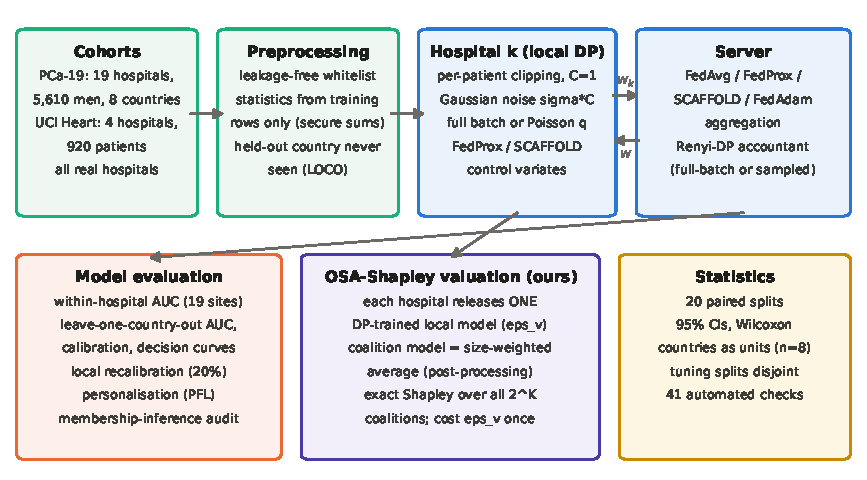
\includegraphics[width=0.85\textwidth]{figures/figure2_architecture.pdf}
    \caption{System architecture. Hospitals train locally with per-patient clipping and Gaussian noise and the server aggregates under a Rényi-DP accountant. The federated model is evaluated within hospitals and on held-out countries (Supplementary Material). Hospitals are valued with OSA-Shapley, which post-processes one DP-trained model per hospital, and compared with retraining and with reconstruction from the training run.}
    \label{fig:architecture}
\end{figure*}


\section{Methods}
\label{sec:method}

\subsection{Classification Model}
Risk is modelled with logistic regression with an intercept,
\begin{equation}
p_i = \sigma(z_i) = \frac{1}{1 + e^{-z_i}}, \qquad z_i = x_i^T w + b,
\end{equation}
trained on binary cross-entropy $\ell(w; x_i, y_i) = - [y_i \ln p_i + (1 - y_i) \ln(1 - p_i)]$ with a small $L_2$ penalty ($\lambda = 10^{-3}$).

\subsection{Rényi Differential Privacy and Sensitivity Analysis}

\subsubsection{Privacy Unit and Adjacency}
We use add/remove adjacency of single records, $D \sim D' \iff |D \triangle D'| = 1$. Every patient contributes one record, so the guarantee is patient-level.

Each per-sample gradient is clipped to $L_2$ norm $C$,
\begin{equation}
\bar{g}_i = g_i / \max\left(1, \frac{\|g_i\|_2}{C}\right),
\end{equation}
so adding or removing one patient changes the summed gradient by at most $C$. The released (noisy) gradient is
\begin{equation}
\tilde{g} = \frac{1}{n_k}\Big(\sum_{i=1}^{n_k} \bar{g}_i + z\Big), \quad z \sim \mathcal{N}\left(0, \sigma^2 C^2 I\right),
\end{equation}
i.e.\ a Gaussian mechanism with noise multiplier $\sigma$ on a sum query of sensitivity $C$ (client sizes $n_k$ are treated as public). The $L_2$ and proximal terms do not access data and are post-processing.

\subsubsection{Rényi DP Composition}
Updates are full-batch (sampling rate $q=1$), so no subsampling amplification is claimed. A Gaussian mechanism with multiplier $\sigma$ satisfies RDP of order $\alpha>1$ with $\epsilon_{RDP}(\alpha) = \alpha/(2\sigma^2)$. Every patient participates in each of the $N = T \times E$ local steps of its own client, and clients hold disjoint patients, so
\begin{equation}
\epsilon = \min_{\alpha \in \mathcal{A}} \left\{ N \cdot \frac{\alpha}{2 \sigma^2} + \frac{\ln(1/\delta)}{\alpha - 1} \right\},
\end{equation}
with a dense order grid $\mathcal{A}$ (1.1--4096). The accountant agrees with the closed-form optimum $\rho + 2\sqrt{\rho \ln(1/\delta)}$, $\rho = N/(2\sigma^2)$, to within 0.01\% and is never below it. For $N=100$ and $\delta=10^{-5}$ the calibrated multipliers are $\sigma = \sigmaTen, \sigmaFive, \sigmaTwo, \sigmaOne, \sigmaHalf$ for $\varepsilon = 10, 5, 2, 1, 0.5$.

Poisson-subsampled DP-SGD with sampled-Gaussian accounting is evaluated as a sensitivity analysis in the Supplementary Material.

\begin{table}[t]
\caption{The privacy cost that retraining-based valuation actually spends (Proposition~2). $r$: number of DP training runs that contain a given hospital's patients (exact Shapley: $2^{K-1}$; permutation sampling without caching: on average $100(K+1)/2$). Each run is $N=100$ full-batch DP-GD steps calibrated to the per-run $\varepsilon$; the table gives the composed $\varepsilon$ per hospital ($\delta=10^{\ensuremath{-}5}$). Last column: factor by which every run's noise must grow to keep the stated budget ($\sqrt r$). Post-processing valuations spend the stated budget once.}
\centering\scriptsize
\setlength{\tabcolsep}{2.5pt}
\resizebox{\columnwidth}{!}{%
\begin{tabular}{lrccccr}
\toprule
 & & \multicolumn{4}{c}{True $\varepsilon$ for a per-run $\varepsilon$ of} & Noise \\
\cmidrule(lr){3-6}
Valuation & $r$ & 10 & 5 & 2 & 1 & factor \\
\midrule
Exact, $K=4$ & 8 & 36 & 16 & 6.1 & 2.9 & 2.8 \\
Exact, $K=10$ & 512 & 988 & 334 & 85 & 33 & 23 \\
Exact, $K=19$ & $\approx 10^{5}$ & $\approx 10^{5}$ & $\approx 10^{5}$ & 23{,}197 & 6{,}116 & 512 \\
Exact, $K=50$ & $\approx 10^{14}$ & $\approx 10^{14}$ & $\approx 10^{14}$ & $\approx 10^{13}$ & $\approx 10^{13}$ & $\approx 10^{7}$ \\
100 permutations, $K=10$ & 550 & 1{,}053 & 354 & 89 & 34 & 23 \\
100 permutations, $K=19$ & 1{,}000 & 1{,}820 & 597 & 141 & 52 & 32 \\
100 permutations, $K=50$ & 2{,}550 & 4{,}464 & 1{,}376 & 303 & 103 & 50 \\
OSA-Shapley, MR, OR (any $K$) & 1 & 10 & 5 & 2 & 1 & 1 \\
\bottomrule
\end{tabular}}
\label{tab:accounting}
\end{table}


\subsection{Exact Shapley Valuation}
The Shapley value of client $k$ is
\begin{equation}
\phi_k = \sum_{S \subseteq \mathcal{N} \setminus \{k\}} \frac{|S|!(K - |S| - 1)!}{K!} \left[ v(S \cup \{k\}) - v(S) \right],
\end{equation}
with $v(\emptyset)=0.5$. We compute it \emph{exactly} by training all $2^K-1$ coalitions (vectorised across coalitions; numerically identical to separate training runs) for $K \le 10$, so no Monte-Carlo error confounds the effect of DP noise. Leave-one-out (LOO) is $v(\mathcal{N}) - v(\mathcal{N}\setminus\{k\})$. Under DP every coalition run draws independent noise. Note that this \emph{retraining} approach releases $2^{K-1}$ privately trained models that involve each hospital; by composition, its total privacy loss is far larger than the per-run $\varepsilon$ (for $K=10$, $N=100$ and a per-run $\varepsilon=1$ it is $\varepsilon\approx\trueEpsOne$; Table~\ref{tab:osa}). We report it because it is the standard way to study valuation under DP, and contrast it with the privacy-honest estimator below.

\subsection{Privacy-Honest Valuation: OSA-Shapley}
\label{sec:osa}
We propose to value hospitals with \emph{one-shot-averaging Shapley} (OSA-Shapley), which spends the privacy budget once:
\begin{enumerate}
\item Each hospital $k$ releases one logistic-regression model $\hat w_k$ trained locally by DP gradient descent at valuation budget $\varepsilon_v$ (\osaSteps{} full-batch steps, per-patient clipping $C=1$, Gaussian noise calibrated with the accountant above). The released model is the average of the iterates of the second half of training, which damps the injected noise.
\item The server forms the model of every coalition as the size-weighted average $w_S = \sum_{k\in S} (n_k/n_S)\,\hat w_k$. For a convex model trained to convergence this one-shot average approximates the FedAvg solution of the coalition; the base paper itself trains its federated models this way.
\item $v(S)$ is the AUC of $w_S$ on the server's reference set, and exact Shapley values follow from all $2^K-1$ utilities by vectorised bitmask summation.
\end{enumerate}
\emph{Assumption.} As for retraining-based valuation, the reference set on which $v(S)$ is computed is held by the server (for example a curated or consented validation set); the guarantees below protect the hospitals' training patients only, not the reference patients (Section~\ref{sec:threats_validity}).

\emph{Proposition 1 (privacy of OSA-Shapley).} If each released model $\hat w_k$ is $(\varepsilon_v,\delta)$-DP with respect to the patients of hospital $k$, then the utilities of all $2^K-1$ coalitions and all Shapley values are jointly $(\varepsilon_v,\delta)$-DP with respect to every training patient, for any $K$.

\emph{Proof.} Hospitals hold disjoint patients, so a single patient affects only one released model; all utilities and Shapley values are deterministic functions of $(\hat w_1,\dots,\hat w_K)$ and the server's reference set. The claim follows from the post-processing property of DP \cite{Dwork2008DPSurvey}. $\square$

\emph{Proposition 2 (cost of retraining-based valuation).} Suppose a valuation trains $r_k$ DP models that each use the patients of hospital $k$, every run consisting of $N$ steps of a full-batch Gaussian mechanism with noise multiplier $\sigma$ (per-run guarantee $(\varepsilon,\delta)$). Then hospital $k$'s total RDP is that of a single run with multiplier $\sigma/\sqrt{r_k}$; equivalently, keeping the total guarantee at $(\varepsilon,\delta)$ requires every run to use multiplier $\sqrt{r_k}\,\sigma$. For exact Shapley values $r_k=2^{K-1}$ (a factor of $22.6$ for $K=10$); for Monte-Carlo permutation sampling with $M$ permutations and no caching, $r_k$ is on average $M(K+1)/2$.

\emph{Proof.} The Gaussian mechanism has RDP $\alpha/(2\sigma^2)$ per step and RDP composes additively, so $r_kN$ steps give $r_kN\alpha/(2\sigma^2) = N\alpha/(2(\sigma/\sqrt{r_k})^2)$; the conversion to $(\varepsilon,\delta)$ depends on the composed RDP only. In a random permutation hospital $k$ is equally likely to be at any of the $K$ positions and joins every prefix from its position on, i.e.\ $(K+1)/2$ of the $K$ prefixes on average. $\square$

Table~\ref{tab:accounting} evaluates Proposition~2. With ten hospitals a per-run $\varepsilon=1$ costs each hospital $\varepsilon\approx\trueEpsOne$; with 19 hospitals exact retraining is out of reach, and even sampling 100 permutations costs $\varepsilon\approx\accMcNineteenOne$. The calibrated multipliers in our experiments follow this ratio exactly (e.g.\ $\sigma=5.68$ per run versus $128.5$ budget-matched at $\varepsilon=10$, $K=10$). If the valuation is released together with the training run, the two budgets compose; OSA-Shapley adds $\varepsilon_v$, retraining adds the much larger composed cost of Proposition~2.

\emph{Approximation.} OSA-Shapley replaces the FedAvg model of each coalition by the average of locally trained models. For i.i.d.\ data and smooth, strongly convex losses such as regularised logistic regression, this average has mean-squared error $O(n^{-1} + (n/m)^{-2})$ for $n$ samples on $m$ sites, matching centralised training when $m \le \sqrt{n}$ \cite{Zhang2013AVGM}. Hospitals are not i.i.d., so we measure the approximation directly: without DP, OSA-Shapley reproduces the retraining Shapley ranking with Spearman $\rho=\osaNoDP$ for the ten largest and \pxSOsaNoDP{} for the ten smallest PCa-19 hospitals (Sections~\ref{sec:p19_osa} and~\ref{sec:p19_small}). \emph{Noise.} Every coalition shares the same released models, so the injected noise is common to all coalitions and largely cancels in marginal contributions. This is the mechanism that Zhou \emph{et al.}\ \cite{Zhou2025Data} exploit by re-using released private gradients, here realised by re-using one released model per hospital in every coalition. \emph{Cost.} Only $K$ local trainings are needed, and the $2^K$ evaluations are cheap: exact Shapley values for all 19 PCa-19 hospitals ($524{,}287$ coalitions) take about a minute on one CPU core. The number of local steps was chosen on four tuning splits that are disjoint from the evaluation splits.

\emph{Proposition 3 (noise of coalition models).} Let each release be $\hat w_k = w_k + \xi_k$, where the DP perturbations $\xi_k$ are independent, zero-mean, and, for $N$ steps of DP gradient descent with step size $\eta$, have per-coordinate standard deviation at most $s_k = \eta\sigma C\sqrt{N}/n_k$ (noise $\mathcal N(0,\sigma^2C^2)$ is added to a gradient sum that is divided by $n_k$; contraction of the loss and iterate averaging only reduce it). Then the perturbation of every coalition model, $\hat w_S - w_S = \sum_{k\in S}(n_k/n_S)\xi_k$, has per-coordinate standard deviation
\begin{equation}
\mathrm{sd}(\hat w_S - w_S) = \frac{1}{n_S}\Big(\sum_{k\in S} n_k^2 s_k^2\Big)^{1/2} \le \frac{\eta\sigma C\sqrt{|S|\,N}}{n_S}.
\label{eq:prop3}
\end{equation}
\emph{Proof.} The $\xi_k$ are independent, so the variance of the weighted sum is $\sum_{k\in S}(n_k/n_S)^2 s_k^2$; substituting the bound on $s_k$ gives $\eta^2\sigma^2C^2 N|S|/n_S^2$. $\square$

Proposition~3 makes two points. First, the noise in a coalition model does not depend on $K$, whereas budget-matched retraining multiplies it by $2^{(K-1)/2}$ (Proposition~2). Second, it shrinks as coalitions grow (for $m$ hospitals of equal size $n$ the bound is $\eta\sigma C\sqrt{N}/(n\sqrt m)$), and it is largest for a single small hospital. OSA-Shapley is therefore accurate when hospitals have hundreds of patients and loses its advantage when they have a few dozen, which is what we observe on the smallest real hospitals (Section~\ref{sec:p19_small}). A validation check confirms the bound empirically (the observed standard deviation is 0.39--0.49 of it).

\emph{Competitors at the same privacy cost.} OSA-Shapley is not the only valuation that is pure post-processing. In DP-FedAvg every hospital releases a noisy local model in every round, and the accountant already covers all $T\cdot E$ steps. Coalition models can therefore be reconstructed from one private training run at no extra cost \cite{Song2019BlockchainFL, Wei2020DataValuation, Liu2022GTG}. We implement the two reconstructions of Song \emph{et al.}\ \cite{Song2019BlockchainFL} exactly. \emph{MR} (multi-round) computes, in every round $t$, exact Shapley values of $v_t(S) = \mathrm{AUC}\big(\sum_{k\in S}(n_k/n_S)\hat w_k^{t}\big)$ with $v_t(\emptyset)$ the AUC of the global model before the round, and sums them over rounds. GTG-Shapley \cite{Liu2022GTG} is a truncated Monte-Carlo approximation of MR, so we evaluate its idealised exact version, MR. \emph{OR} (one-round) rebuilds $w_S = w^0 + \sum_t\sum_{k\in S}(n_k/n_S)(\hat w_k^{t} - w^{t-1})$ from the accumulated updates. Both use the same DP-FedAvg run, at the same $\varepsilon$, as the federated model.

\emph{Cheap proxies.} To test whether a valuation protocol is needed at all, we compare OSA-Shapley with scores that hospitals could share more cheaply: (i) hospital size $n_k$; (ii) the number of cancer cases; (iii) the similarity of summary statistics, the negative distance between a hospital's feature means and prevalence and the pooled ones; (iv) a self-reported AUC of the hospital's own model on its own test patients; (v) the AUC of its single released DP model on the reference set; and (vi) the leave-one-out value of the averaged releases, $v(\mathcal N)-v(\mathcal N\setminus\{k\})$. Proxies (v) and (vi) use exactly the releases of OSA-Shapley and therefore cost the same $\varepsilon$; proxies (i)--(iii) are shared without DP and (iv) cannot be verified by the server.

\emph{Accuracy.} We compare each valuation's ranking with the exact non-private retraining Shapley ranking by Spearman's $\rho$ and report how often a hospital with random labels is ranked last.

\subsection{Statistical Analysis}
Every experiment is repeated over 20 seeds. A seed re-draws the stratified 80/20 split within every hospital, model noise and DP noise, so seed-to-seed variation covers all sources of randomness. We report means with $t$-based 95\% confidence intervals over seeds. Comparisons between methods are \emph{paired} by seed; we report the mean paired difference with its 95\% CI and a two-sided Wilcoxon signed-rank test, and call a difference significant only if its CI excludes zero.

\section{Data and Protocol}
\label{sec:data}

\subsection{PCa-19: The Base Paper's 19 Hospitals}
PCa-19 is the patient-level collection used by the base paper, released in the authors' public repository (MIT licence) \cite{Kazlouski2025HospitalParticipation}. The authors harmonised it from the supplementary files of 19 peer-reviewed prostate-cancer studies. It contains \pNineN{} men from \pNineHosp{} hospitals (Table~\ref{tab:pca19_cohort}); \pNinePos{} (\pNinePrev\%) have clinically significant cancer (csPCa, ISUP grade group $\geq 2$ at biopsy), ranging from \pNinePrevLo\% to \pNinePrevHi\% per hospital. The base paper's text states nine countries, but its Table~I and the released data contain eight (Spain, South Korea, Germany, China, USA, Netherlands, Italy, UK); we use the released data unchanged. Every variable is available before biopsy: age, PSA, prostate volume (PV) and the highest PI-RADS score. (A 5-$\alpha$-reductase-inhibitor flag is 0 for all patients and is not used.) Our feature set is age, $\log$ PSA, $\log$ PV and indicators for PI-RADS 3, 4 and 5. The logarithms keep the extreme PSA values of one hospital (median 277~ng/mL) from dominating, and standardisation statistics are computed from training rows only. For the reproduction of the authors' protocol we use their exact Ettala and Noh variables.



\subsection{Second Federation: UCI Heart Disease}
\label{sec:heart_data}
The UCI Heart Disease collection \cite{Janosi1988HeartDisease, Detrano1989Heart} contains \hrN{} patients referred for coronary angiography at four hospitals: the Cleveland Clinic Foundation (USA, 303), the Hungarian Institute of Cardiology in Budapest (294), the University Hospitals of Zurich and Basel (123) and the VA Medical Center in Long Beach (USA, 200). It is a standard real-silo benchmark for federated learning \cite{Terrail2022FLamby}. The target is angiographic coronary artery disease (any vessel narrowed by more than 50\%), whose prevalence ranges from 36\% (Budapest) to 93\% (Switzerland). We drop the three variables with more than 30\% missing values (slope, number of vessels, thallium test), treat a cholesterol of zero as missing (all Swiss patients), impute remaining gaps with the median of the pooled training rows plus a missingness indicator, one-hot encode chest-pain type and resting ECG, and standardise with training-row statistics, giving \hrFeat{} features. OSA-Shapley keeps the hyper-parameters chosen on PCa-19, so this cohort is an out-of-sample test of the method as well as of the decision rule.

\subsection{Silos, Splits and Reference Sets}
\label{sec:silos}
Every client is a real hospital exactly as released (one of the 19 PCa-19 hospitals or the four heart-disease hospitals); we never simulate hospitals or partition a pooled data set, so every valued unit is an institution that could join a federation. Within each hospital patients are split 80/20 into training and test sets, stratified by outcome, and a new split is drawn for every seed. We value two groups for which the exact non-private reference is computable (all $2^{10}-1$ coalitions retrained): the ten largest hospitals (266--763 patients; the Dutch hospital, the tenth largest, also belongs to the smallest ten) and the ten smallest (\pxSmallMin--\pxSmallMax{} patients; \pxSmallHosp). All 19 hospitals are valued with OSA-Shapley only, because no exact reference exists for them. In the heart-disease federation all four hospitals are valued against the exact reference ($2^4-1$ coalitions). The reference set on which $v(S)$ is scored is the pooled test patients of the valued hospitals and is never used for training. The only controlled perturbation is the ``useless hospital'' of Section~\ref{sec:p19_robust}, a real hospital whose training labels are replaced by random labels at its own prevalence (\corrHosp{} in PCa-19, \hrCorrupt{} in the heart-disease federation).

\subsection{Protocol}
Unless stated otherwise: $T=20$ rounds, $E=5$ local epochs ($N=100$ steps), learning rate $\eta=0.5$, $\lambda=10^{-3}$, $\mu=0.5$, $C=1$, $\delta=10^{-5}$, 20 seeds. These optimiser settings were fixed before the valuation experiments and are shared by every method; OSA-Shapley's single hyper-parameter (the number of local steps) was chosen on four tuning splits.



Valuation experiments use 20 further splits (seeds 20--39) that were not used for any tuning.

\section{Results}
\label{sec:results}
All results use real hospitals as released: the 19 PCa-19 hospitals and, in Section~\ref{sec:heart}, the four heart-disease hospitals. We first summarise the federation that is valued (Section~\ref{sec:federation}); its full analysis is in Supplementary Section~\ref{sec:pca19_more}. We then turn to valuation under DP (Sections~\ref{sec:p19_retrain}--\ref{sec:heart}).

\subsection{The Federation Being Valued}
\label{sec:federation}
Our re-implementation of the base paper's protocol reproduces the authors' released code to within $1.2\times10^{-14}$ for both of their calculators (Supplementary Section~\ref{sec:p19_repro}), and its sustainability finding holds under our protocol: joining brings no significant average gain over local training (FL$-$LOC $=\pDFLminusLOC$), a free-rider obtains almost the same model (FR$-$FL $=\pDFRminusFL$), and federated training matches pooled training (CEN$-$FL $=\pDCENminusFL$). For this seven-parameter, regularised logistic calculator trained on \pNineN{} patients, DP changes the mean per-hospital AUC by only $\pDpLossHalf$ even at $\varepsilon=0.5$. We do not generalise this: the cost of a given $\varepsilon$ depends strongly on the model and the amount of data, and for a federated MLP the same budgets perturb the released models far more (Section~\ref{sec:p19_mlp}). Discrimination transports to held-out countries, but calibration does not (observed/expected ratios \pOeMin--\pOeMax); an intercept update on 20\% of a new country's patients, which is common clinical practice for risk calculators anyway, reduces $|\log\mathrm{O/E}|$ from \pRecalOeRaw{} to \pRecalOeInt{} (Supplementary Section~\ref{sec:p19_loco}).

\subsection{Retraining-Based Valuation under DP}
\label{sec:p19_retrain}
Following standard practice, we first retrain every coalition with DP at a per-run $\varepsilon$ and compute exact Shapley values over the ten largest hospitals (1{,}023 coalitions). Their agreement with the non-private ranking falls from Spearman $\rho=\pShRhoTen$ at $\varepsilon=10$ to \pShRhoTwo{} at $\varepsilon=2$ and \pShRhoHalf{} at $\varepsilon=0.5$ (original splits, against the no-DP ranking; Table~\ref{tab:osa} repeats this on the held-out splits against exact Shapley), although the federation's AUC changes by less than 0.01 over this range. Leave-one-out values are near zero for every hospital and cannot separate contributors (Spearman with Shapley \pShLooRho). These results ignore the cost of the valuation itself.

\subsection{Valuation at an Honest Privacy Budget}
\label{sec:p19_osa}
Table~\ref{tab:osa} makes the real cost of retraining explicit: with ten hospitals each hospital joins 512 private training runs, so a per-run $\varepsilon$ of 10, 5 or 1 corresponds to a total $\varepsilon$ of about \trueEpsTen{}, \trueEpsFive{} and \trueEpsOne{} per hospital. When the total budget is held at the stated $\varepsilon$ (\emph{budget-matched} retraining), every run needs much more noise and the ranking is lost: Spearman $\rho$ with the exact non-private Shapley values falls to \bmRhoTen{} at $\varepsilon=10$ and \bmRhoOne{} at $\varepsilon=1$.

OSA-Shapley (Section~\ref{sec:osa}) spends the budget once. Without DP it reproduces the retraining Shapley ranking almost exactly ($\rho=\osaNoDP$), and under DP it keeps $\rho=\osaRhoTen$ at $\varepsilon=10$, \osaRhoTwo{} at $\varepsilon=2$, \osaRhoOne{} at $\varepsilon=1$ and \osaRhoHalf{} at $\varepsilon=0.5$ (Table~\ref{tab:osa}; evaluated on 20 splits that were not used to choose its single hyper-parameter). At equal privacy it beats retraining by $\osaVsBmTwo$ in $\rho$ at $\varepsilon=2$. At $\varepsilon=2$ it matches per-run retraining ($\osaVsPrTwo$), which spends 28--42 times more privacy. Because no coalition needs training, exact valuation of all 19 hospitals is feasible: the OSA ranking computed with DP agrees with the non-private one at $\rho=\osaNineRhoFive$ ($\varepsilon=5$) and \osaNineRhoOne{} ($\varepsilon=1$).


\subsection{Against Valuations that Also Cost the Budget Once}
\label{sec:p19_post}
The fair competitors are the reconstruction methods MR and OR, which post-process the DP-FedAvg run (Section~\ref{sec:osa}). Table~\ref{tab:osa_post} and Fig.~\ref{fig:osa} compare them on the same splits. For the ten largest hospitals, OSA-Shapley is more accurate than exact MR, the upper bound for GTG-Shapley, at every privacy level: $\rho$ \osaRhoTwo{} vs \mrRhoTwo{} at $\varepsilon=2$ (difference \osaVsMrTwo) and \osaRhoOne{} vs \mrRhoOne{} at $\varepsilon=1$ (\osaVsMrOne). It also beats OR by \osaVsOrTwo{} at $\varepsilon=2$. The gap is already present without DP ($\rho$ \osaNoDP{} vs \mrRhoNoDP), so it comes from the coalition proxy rather than from the noise.


\subsection{Is OSA-Shapley Worth It? Cheap Proxies}
\label{sec:p19_proxies}
A federation could avoid a valuation protocol altogether and credit hospitals by what they can share cheaply. Table~\ref{tab:proxies} compares these proxies with OSA-Shapley against the same exact non-private reference. For the ten largest hospitals, hospital size, the number of cancer cases and the similarity of summary statistics to the pooled ones carry almost no information about contribution ($\rho$ \pxLSizeNoDP, \pxLPosNoDP{} and \pxLStatNoDP; OSA$-$size $=\pxdLSizeTwo$ at $\varepsilon=2$). They also cannot detect a hospital with useless data, because random labels change neither its size nor its prevalence (0\% of splits). Hospitals here differ in case mix, not only in size, and their marginal value depends on what the other hospitals already provide. An AUC that each hospital reports for its own model is unverifiable and agrees poorly with the ranking ($\rho=\pxLOwnTwo$ at $\varepsilon=2$).

Proxies built on a released model behave differently. Once each hospital has released one DP model, as OSA requires, the AUC of that single model on the reference set already ranks the large hospitals well ($\rho=\pxLRefTwo$ at $\varepsilon=2$) and flags the useless hospital. OSA-Shapley is comparable at $\varepsilon=2$ ($\pxdLRefTwo$) and better at $\varepsilon=1$ ($\pxdLRefOne$), where single releases are noisy and averaging over coalitions helps; it also beats the leave-one-out value of the averaged releases by $\pxdLLooTwo$. Both scores use the same releases, so OSA's advantage costs no extra privacy or communication. OSA's values are also Shapley values: they sum to the federation's gain over chance, which a single-model score does not.

On the ten smallest hospitals the picture changes (Table~\ref{tab:proxies}, right). There contribution is driven mainly by data volume, and hospital size alone reaches $\rho=\pxSSizeNoDP$. At $\varepsilon=2$, OSA-Shapley, MR, the single-model score and size agree with the ranking about equally well (OSA$-$size $=\pxdSSizeTwo$, OSA$-$MR $=\pxdSMrTwo$), and at $\varepsilon=1$ none of the DP valuations is better than size.

\begin{table*}[t]
\caption{Is OSA-Shapley worth its cost? Agreement (Spearman $\rho$) of cheap contribution proxies and of privacy-honest valuations with the exact non-private retraining Shapley ranking, on real PCa-19 hospitals (20 held-out splits). \emph{What is shared}: what each hospital must reveal. Proxies that use a model use the same DP releases as OSA-Shapley and therefore cost the same $\varepsilon$; size, counts and statistics are shared without DP. \emph{Useless}: share of splits in which a hospital whose training labels were replaced by random labels (es6) is ranked last at $\varepsilon=2$; a tie for last place does not count.}
\centering\scriptsize
\setlength{\tabcolsep}{4pt}
\begin{tabular}{llccccccc}
\toprule
 & & \multicolumn{4}{c}{Ten largest hospitals} & \multicolumn{3}{c}{Ten smallest hospitals} \\
\cmidrule(lr){3-6}\cmidrule(lr){7-9}
Contribution score & What is shared & no DP & $\varepsilon=2$ & $\varepsilon=1$ & Useless & no DP & $\varepsilon=2$ & $\varepsilon=1$ \\
\midrule
Hospital size $n_k$ & size (public) & 0.08 & 0.08 & 0.08 & 0\% & 0.74 & 0.74 & 0.74 \\
Number of csPCa cases & one count & 0.02 & 0.02 & 0.02 & 0\% & 0.50 & 0.50 & 0.50 \\
Similarity of summary statistics & feature means, prevalence & \ensuremath{-}0.18 & \ensuremath{-}0.18 & \ensuremath{-}0.18 & 0\% & 0.72 & 0.72 & 0.72 \\
Self-reported local AUC & one AUC (unverifiable) & 0.36 & 0.25 & 0.26 & 100\% & 0.40 & 0.54 & 0.56 \\
Single-model AUC on reference set & one DP model ($\varepsilon$) & 0.93 & 0.85 & 0.71 & 100\% & 0.94 & 0.79 & 0.72 \\
Leave-one-out of averaged models & one DP model ($\varepsilon$) & 0.85 & 0.77 & 0.74 & 0\% & 0.59 & 0.34 & 0.34 \\
OR reconstruction & DP-FedAvg run ($\varepsilon$) & 0.42 & 0.51 & 0.50 & 100\% & 0.79 & 0.74 & 0.59 \\
MR reconstruction (GTG bound) & DP-FedAvg run ($\varepsilon$) & 0.74 & 0.75 & 0.65 & 70\% & 0.86 & 0.78 & 0.74 \\
Retraining, budget-matched & $2^{K-1}$ runs ($\varepsilon$) & -- & 0.18 & 0.10 & 60\% & -- & 0.45 & 0.29 \\
\textbf{OSA-Shapley (ours)} & one DP model ($\varepsilon$) & \textbf{0.96} & \textbf{0.89} & \textbf{0.80} & 100\% & \textbf{0.95} & \textbf{0.79} & \textbf{0.68} \\
\bottomrule
\end{tabular}
\label{tab:proxies}
\end{table*}


\subsection{A Hospital with Useless Data, Removal and Robustness}
\label{sec:p19_robust}
We replaced the training labels of one mid-sized hospital (\corrHosp) by random labels and asked whether each valuation ranks it last (Tables~\ref{tab:proxies} and~\ref{tab:osa_robust}). The non-private retraining Shapley values always do (\corrTruth). At $\varepsilon=2$ and $\varepsilon=1$, OSA-Shapley ranks it last in \corrOsaTwo{} and \corrOsaOne{} of splits, MR in \corrMrTwo{} and \corrMrOne, and budget-matched retraining in only \corrBmTwo{} and \corrBmOne; no size- or statistics-based proxy ever does. Sensitivity to the reference-set size and the number of local steps is reported in Table~\ref{tab:osa_robust}.

\subsection{A Non-Convex Model}
\label{sec:p19_mlp}
OSA-Shapley assumes that averaging locally trained models approximates the federated model of a coalition, which holds for convex losses. We therefore repeated the comparison with a one-hidden-layer MLP (16 tanh units) trained by FedAvg, with exact non-private retraining Shapley values of the federated MLP as the reference (Table~\ref{tab:osa_mlp}). Because averaging the parameters of separately trained networks is fragile, the coalition prediction is the size-weighted average of the members' log-odds (OSA-ens.), which is equally post-processing. Without DP the ensemble variant reproduces the reference ranking well ($\rho=\mlpOsaNoDP$, against \mlpMrNoDP{} for MR). Under DP it loses this advantage: at $\varepsilon=2$ and $\varepsilon=1$ it reaches \mlpOsaTwo{} and \mlpOsaOne{}, whereas MR reaches \mlpMrTwo{} and \mlpMrOne{} (OSA$-$MR $=\mlpOsaVsMrTwo$ at $\varepsilon=2$). A non-linear model trained alone for 200 noisy steps accumulates the DP perturbation, whereas MR's short local updates restart from the shared global model in every round. Budget-matched retraining of the MLP is close to chance ($\rho=\mlpBmTwo$; \mlpBmSeeds{} splits). For non-convex models, reconstruction from the training run is the better privacy-honest valuation.


\subsection{Small Hospitals: Where OSA-Shapley Loses Its Advantage}
\label{sec:p19_small}
To study small silos without simulating any, we value the ten smallest PCa-19 hospitals (\pxSmallMin--\pxSmallMax{} patients; exact non-private retraining Shapley as reference, 20 held-out splits). Without DP, OSA-Shapley is again the most accurate valuation ($\rho=\pxSOsaNoDP$; OSA$-$MR $=\pxdSMrNoDP$). Under DP its advantage disappears: at $\varepsilon=2$ OSA and MR agree with the ranking equally well (\pxSOsaTwo{} and \pxSMrTwo{}; difference $\pxdSMrTwo$), and at $\varepsilon=1$ MR is slightly, not significantly, ahead (\pxdSMrOne). Budget-matched retraining remains far worse ($\rho=\pxSBmTwo$ at $\varepsilon=2$). This is the regime that Proposition~3 predicts: the release of a hospital with a few dozen patients carries noise of order $\sigma/n_k$, whereas reconstruction averages over the federation in every round. With hospitals this small, hospital size is itself a strong proxy (Section~\ref{sec:p19_proxies}), and no privacy-honest valuation improves on it at $\varepsilon \le 1$.


\subsection{A Second Real Federation: Heart Disease}
\label{sec:heart}
Table~\ref{tab:heart} repeats the comparison on the four hospitals of the UCI Heart Disease collection, with OSA-Shapley's PCa-19 hyper-parameters unchanged. Without DP the picture is the same as before: OSA-Shapley recovers the exact ranking best ($\rho=\hrOsaNoDP$, against \hrMrNoDP{} for MR and \hrRefNoDP{} for the single-model score; OSA$-$MR $=\hrdMrNoDP$). Under DP it is not. These hospitals have 98--242 training patients for 21 model parameters, and their contributions are nearly equal (Shapley values \hrPhiMin--\hrPhiMax{} AUC), so the noise of a single release dominates. At $\varepsilon=5$ OSA-Shapley and MR are close (\hrOsaFive{} and \hrMrFive{}); at $\varepsilon=2$ MR is better (\hrMrTwo{} vs \hrOsaTwo{}; OSA$-$MR $=\hrdMrTwo$); and at $\varepsilon=1$ no valuation agrees with the ranking beyond chance. Retraining does not help: with four hospitals its composed cost is modest (a stated $\varepsilon=2$ really costs \hrTrueTwo), yet per-run and budget-matched retraining reach only \hrPrTwo{} and \hrBmTwo{}. Hospital size is anti-correlated with contribution ($\rho=\hrSizeNoDP$): the smallest hospital, Zurich/Basel, contributes most. Released models still detect bad data: OSA-Shapley and the single-model score rank \hrCorrupt{} with random labels last in \hrCOsaTwo{} and \hrCRefTwo{} of splits at $\varepsilon=2$, hospital size in \hrCSizeTwo.

\begin{table}[t]
\caption{Second real federation: the four hospitals of the UCI Heart Disease collection (Cleveland (303), Budapest (294), Zurich/Basel (123), Long Beach VA (200) patients), coronary artery disease, 20 held-out splits. Spearman $\rho$ with the exact non-private retraining Shapley ranking; with four hospitals $\rho$ moves in steps of 0.2. Per-run retraining really costs $\varepsilon\approx16$, 6.1 and 2.9 at a stated 5, 2 and 1. \emph{Useless}: share of splits in which Budapest, given random training labels, is ranked last at $\varepsilon=2$.}
\centering\scriptsize
\setlength{\tabcolsep}{3pt}
\begin{tabular}{lccccc}
\toprule
Contribution score & no DP & $\varepsilon=5$ & $\varepsilon=2$ & $\varepsilon=1$ & Useless \\
\midrule
Hospital size $n_k$ & \ensuremath{-}0.38 & \ensuremath{-}0.38 & \ensuremath{-}0.38 & \ensuremath{-}0.38 & 0\% \\
Similarity of summary statistics & \ensuremath{-}0.38 & \ensuremath{-}0.38 & \ensuremath{-}0.38 & \ensuremath{-}0.38 & 0\% \\
Self-reported local AUC & \ensuremath{-}0.18 & \ensuremath{-}0.17 & \ensuremath{-}0.31 & \ensuremath{-}0.30 & 70\% \\
Single-model AUC on reference set & 0.76 & 0.42 & \ensuremath{-}0.04 & \ensuremath{-}0.34 & 100\% \\
Leave-one-out of averaged models & 0.82 & 0.69 & 0.42 & 0.18 & 85\% \\
OR reconstruction & 0.23 & 0.29 & 0.18 & 0.04 & -- \\
MR reconstruction (GTG bound) & 0.70 & 0.64 & 0.45 & \ensuremath{-}0.35 & -- \\
Retraining, per run & -- & 0.34 & \ensuremath{-}0.09 & \ensuremath{-}0.27 & -- \\
Retraining, budget-matched & -- & \ensuremath{-}0.02 & \ensuremath{-}0.18 & \ensuremath{-}0.15 & -- \\
\textbf{OSA-Shapley (ours)} & \textbf{0.92} & \textbf{0.51} & \textbf{0.15} & \textbf{\ensuremath{-}0.18} & 100\% \\
\bottomrule
\end{tabular}
\label{tab:heart}
\end{table}


\section{A Decision Rule, Tested in Advance}
\label{sec:rule}
\subsection{The Index and the Original Rule}
Supplementary Table~\ref{tab:decision} puts the four settings side by side. By Proposition~3 the per-coordinate noise of a release scales as $1/n_k$, so its norm over $p$ parameters scales as $\sqrt p/n_k$; we therefore index a setting by $\nu$, the median number of training patients per hospital divided by $\sqrt p$. In these settings OSA-Shapley won at $\nu=\nuLarge$ (ten largest PCa-19 hospitals) and did not at $\nu\le\nuSmall$ (ten smallest: \nuSmall; heart disease: \nuHeart; MLP: \nuMlp), which suggested a switch-over between $\nu\approx50$ and 100.

\subsection{A Pre-Registered Test}
A threshold read off the same results it explains is not evidence, so we tested it on new conditions. Before running anything, we wrote down the design and six hypotheses and fixed them with a cryptographic hash (Supplementary Section~\ref{sec:prereg}); the protocol was registered internally, not on a public registry, and written and run on the same day, so its timing cannot be verified independently; we treat the test as a prospectively specified internal check rather than a formal pre-registration. Within the ten largest PCa-19 hospitals we lowered $\nu$ in two ways: arm A keeps 60\% to 15\% of every hospital's training patients, and arm B adds 21 to 100 uninformative features; in each condition the reference is the exact non-private retraining Shapley ranking of that condition (Fig.~\ref{fig:nu}, Table~\ref{tab:nu_sweep}).

The direction of the rule held, but its threshold did not. As predicted, OSA-Shapley beat MR at $\nu\ge100$ (H1), its advantage shrank with $\nu$ (H3; Spearman correlation \nsSpear{}), both arms agreed in sign at matched $\nu$ (H5), and stronger privacy moved the switch-over to higher $\nu$ (H6). Contrary to H2 and H4, OSA-Shapley kept a significant advantage down to $\nu\approx\nsAFortyFiveNu$ (OSA$-$MR $=\nsAFortyFiveTwo$ at $\varepsilon=2$), tied with MR at $\nu\approx30$--57 when parameters were added, and fell behind only at $\nu\approx\nsASeventeenNu$ (OSA$-$MR $=\nsASeventeenTwo$ at $\varepsilon=2$, $\nsASeventeenOne$ at $\varepsilon=1$). The mean difference changed sign at $\nu\approx\nsCrossTwo$ for $\varepsilon=2$ and between \nsCrossOneMin{} and \nsCrossOneMax{} for $\varepsilon=1$, not between 50 and 100. Two of the six hypotheses therefore failed, and we revise the rule accordingly.

\begin{figure}[!t]
\centering
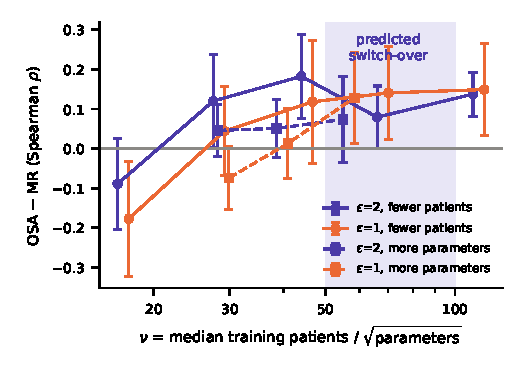
\includegraphics[width=\columnwidth]{figures/figure20_nu_sweep.pdf}
\caption{Internally pre-registered test: OSA$-$MR (paired difference in Spearman $\rho$ with the exact reference, 95\% CI, 20 splits) as $\nu$ is lowered within the ten largest PCa-19 hospitals, by removing patients (solid) or adding uninformative parameters (dashed). Shaded: the switch-over predicted before the test. Points at the same $\nu$ are offset slightly for legibility.}
\label{fig:nu}
\end{figure}

\subsection{The Revised Rule}
\begin{enumerate}
    \item \emph{Count the cost.} Report the composed $\varepsilon$ of any valuation (Proposition~2) and do not retrain coalitions at a per-run budget; retraining was not accurate in any setting.
    \item \emph{Without DP on the releases} (for example, when model sharing is covered by a data-use agreement), use OSA-Shapley, the most accurate valuation in all four settings ($\rho$ \mlpOsaNoDP--\osaNoDP).
    \item \emph{Under DP with a convex model}, OSA-Shapley is at least as accurate as MR down to $\nu\approx30$ at $\varepsilon=2$ and $\nu\approx40$ at $\varepsilon=1$; below that, use MR, which adds no privacy cost when the federation already trains with DP-FedAvg.
    \item \emph{With a non-convex model}, use MR.
    \item \emph{Check hospital size before using it.} Size matched contribution only where hospitals differed mainly in volume (\pxSSizeTwo{} for the ten smallest PCa-19 hospitals) and failed elsewhere (\pxLSizeTwo{} and \hrSizeTwo). Neither size nor summary statistics can detect bad data; the score of a single released model can.
    \item \emph{Compute both OSA-Shapley and MR when in doubt.} $\nu$ does not explain every case: the heart-disease federation ($\nu=\nuHeart$) favoured MR although the sweep says OSA should be competitive there. Its four hospitals make $\rho$ coarse, and site-specific missing data make some features constant within a hospital, so single-hospital models are poorly determined; both explanations are untested. Disagreement between the two valuations is a sign that the ranking is not resolved at the chosen budget, and with small $\nu$ at $\varepsilon\le1$ coarse credit (equal shares plus screening for bad data) is the honest fallback.
\end{enumerate}


\section{Discussion}
\label{sec:discussion}
The main lesson is about accounting. Studies of contribution valuation under DP routinely report a per-run privacy budget, but a hospital whose data enter $2^{K-1}$ coalition runs pays for all of them. On ten real hospitals that turns a stated $\varepsilon=1$ into $\varepsilon\approx\trueEpsOne$, and when the budget is held honestly the ranking collapses. Any payment, reputation or cost-sharing scheme built on such valuations either over-spends privacy or rewards the wrong hospitals. The remedy is to restrict valuation to post-processing of releases whose cost is already counted.

\emph{Is it practical?} OSA-Shapley asks each hospital for one DP-trained model, here seven numbers, which is the size of a single update in the 20-round DP-FedAvg run that the federation performs anyway; the $2^K$ coalition evaluations happen on the server and take about a minute for 19 hospitals. The cheaper alternative of sharing sizes, case counts or summary statistics is unreliable: these proxies were essentially uninformative for the large prostate-cancer hospitals ($\rho\le\pxLSizeNoDP$), anti-correlated with contribution in the heart-disease federation ($\rho=\hrSizeNoDP$), and blind to a hospital with useless data, because what a hospital adds depends on its case mix relative to the others, not on its size. Once a hospital has released a model, a single-model score is a reasonable approximation, which OSA-Shapley improves on at no extra privacy cost ($\pxdLRefOne$ at $\varepsilon=1$) while yielding proper Shapley values.

Within the privacy-honest class no single method is best, and Section~\ref{sec:rule} turns our evidence into a rule. Its mechanism is simple: a valuation built on single releases is as good as those releases, whose noise grows with the number of parameters and shrinks with the number of patients, whereas reconstruction trades some bias (reconstructed models carry information from hospitals outside the coalition) for averaging over the whole federation in every round. Which effect dominates depends mainly on $\nu$, although $\nu$ did not explain the heart-disease result (Section~\ref{sec:rule}).

We avoid general statements about $\varepsilon$: the same budget barely changes the seven-parameter prostate calculator but degrades the heart-disease model and the MLP considerably, so results must be read per model and data size. Calibration, finally, is a local matter: the federated calculator transports in discrimination but not in calibration, and recalibrating the intercept on a hospital's own patients, already common practice before a risk calculator is used, removes most of the miscalibration (Supplementary Material).

\subsection{Threats to Validity}
\label{sec:threats_validity}
\emph{Internal.} OSA-Shapley's local steps were tuned on four splits and evaluated on twenty disjoint ones. The reference for valuation accuracy is exact non-private retraining Shapley over the ten largest and the ten smallest PCa-19 hospitals and all four heart-disease hospitals; for all 19 hospitals no exact retraining reference exists, so we report agreement with the non-private OSA ranking. PCa-19 data were harmonised by the base paper's authors from published supplementary files, and two hospitals have fewer than 50 patients.

\emph{External.} All evaluations are retrospective and use two federations and two clinical tasks; with four hospitals, Spearman $\rho$ moves in steps of 0.2, so the heart-disease estimates are coarse. One-shot averaging approximates the federated solution well for regularised logistic regression; for a federated MLP it is accurate without DP but loses to reconstruction under DP, and deeper networks are untested. All models are low-dimensional tabular models (logistic regression with 7--107 parameters and a 16-unit MLP); for imaging or other deep models $\nu$ is orders of magnitude smaller, our results suggest that OSA-Shapley would not be the right choice there, and the rule has not been tested in that regime. Shapley values depend on the reference population on which coalitions are scored, and we have not tested a reference set from outside the federation.

\emph{Privacy.} The guarantee is per patient and treats hospital sizes and shared preprocessing statistics as public. OSA-Shapley's guarantee covers the valuation release; if the training run is also released, the two budgets compose. Like every Shapley method, it scores coalitions on a reference set held by the server, and the patients of that set are not protected: every utility $v(S)$ is a deterministic function of their records. Our experiments use the pooled test patients in this role, which is more than a real server would hold. In deployment the reference set should be public, consented for this use or itself privately released, or the utilities should be released with their own DP noise, whose cost then composes with $\varepsilon_v$; we have not evaluated these options. The main experiments use full-batch updates with conservative accounting.

\emph{Statistical.} Comparisons are paired over 20 splits that share the same patients, so CIs describe variability across splits rather than across federations.

\subsection{Data, Code, Ethics and Conflicts}
Both data sets are public and were used as released: PCa-19 from the base study's repository \cite{Kazlouski2025HospitalParticipation} and the UCI Heart Disease collection (doi:10.24432/C52P4X) \cite{Janosi1988HeartDisease}. They are de-identified, and no new patient data were collected, so no ethics approval was required. The authors declare no conflicts of interest and received no external funding. All results, tables and figures are regenerated from code: \texttt{python run\_pca19.py} recomputes every experiment, \texttt{python -m fl\_study.validate} runs 41 automated checks (data integrity, agreement with the base paper's code, the accountants, Propositions~2 and~3, and absence of leakage), and \texttt{python Paper/generate\_paper\_assets.py} writes every number in this manuscript. Code: \url{https://github.com/JeyanthPonnaluri/Mini_Project_RVR}.

\section{Conclusion}
\label{sec:conclusion}
Valuing hospitals by retraining coalitions under differential privacy spends the privacy budget hundreds of times over, and at an honest budget it loses the contribution ranking; Monte-Carlo sampling reduces this cost only for large federations and never removes it. Valuation should therefore post-process releases whose cost is already counted. Among such valuations none wins everywhere. On two real federations, OSA-Shapley, which averages one DP-trained model per hospital, is the most accurate without DP and, under DP, when hospitals hold many patients per model parameter; reconstruction from the training run is better for a neural network and in the heart-disease federation, an exception the rule does not yet explain; hospital size and summary statistics are unreliable and cannot detect bad data. Patients per hospital relative to the square root of the model's parameters predicts the choice in direction; an internally pre-registered test moved the switch-over to about 30 at $\varepsilon=2$ and 40 at $\varepsilon=1$, and a federation near it should compute both valuations and report the composed privacy cost of whatever it runs. OSA-Shapley should be read as a strong baseline for low-dimensional convex models, not as a general method. Explaining the heart-disease exception, testing the revised rule on a new federation under a public pre-registration, OSA variants for neural networks, and prospective incentive schemes are the next steps.

\bibliographystyle{IEEEtran}
\bibliography{references}

\clearpage
\onecolumn
\begin{center}{\Large\bfseries Supplementary Material}\end{center}
\twocolumn
\setcounter{section}{0}\setcounter{table}{0}\setcounter{figure}{0}\setcounter{equation}{0}
\renewcommand{\thetable}{S\arabic{table}}
\renewcommand{\thefigure}{S\arabic{figure}}
\renewcommand{\thesection}{S\arabic{section}}
\renewcommand{\theequation}{S\arabic{equation}}


This supplement contains additional methods, the reproduction of the base paper, the full analyses of the federation that is valued (federated training, differential privacy, transport and calibration; summarised in Section~\ref{sec:federation} of the main paper), detailed tables, and all claims with verdicts computed from the result files. All analyses use real hospitals as released (the 19 PCa-19 hospitals and the four UCI Heart Disease hospitals); no hospital is simulated and no data set is partitioned artificially. Numbers without the prefix ``S'' refer to the main paper.

\section{Additional Methods}
\label{sec:methods_more}
\subsection{Subsampled Accounting}
As an alternative we also train with Poisson subsampling: in every local step each patient is included independently with probability $q<1$, the clipped gradients of the included patients are summed, noise $\mathcal{N}(0,\sigma^2C^2I)$ is added and the sum is divided by the \emph{expected} batch size $q\,n_k$; $1/q$ steps make one epoch, so $N = T\,E/q$. One step is then a sampled Gaussian mechanism, whose RDP at integer order $\alpha$ is \cite{Mironov2019SampledGaussian, Zhu2019Poisson, Wang2019SubsampledRDP}
\begin{equation}
\epsilon_{RDP}(\alpha) = \frac{1}{\alpha-1}\ln \sum_{j=0}^{\alpha} \binom{\alpha}{j} (1-q)^{\alpha-j} q^{j} \exp\!\Big(\frac{j^2-j}{2\sigma^2}\Big),
\end{equation}
composed over the $N$ steps and converted as above (orders 2--1024). For $q=1$ it reduces to $\alpha/(2\sigma^2)$. Our implementation matches a numerical evaluation of the Rényi divergence to $10^{-13}$ and reproduces the value $\varepsilon \approx 1.26$ reported by Abadi \emph{et al.}\ \cite{Abadi2016DPSGD} for $q=0.01$, $\sigma=4$, $10{,}000$ steps and $\delta=10^{-5}$. Subsampling lowers the noise multiplier required for a given $\varepsilon$ (privacy amplification \cite{Balle2018Amplification}) at the price of more, smaller-batch steps; whether this improves utility is an empirical question (Section~\ref{sec:p19_subsampling}).

\subsection{Membership Inference Attack Formulation}
We audit empirical leakage with a confidence-threshold membership-inference attack. The score of a record is the model's confidence in its true label, $s_i = y_i p_i + (1 - y_i)(1 - p_i)$. Members (training patients) are subsampled to the number of non-members (test patients) and the attack is summarised by its ROC AUC. As a positive control, the same attack is applied to a deliberately over-fitted model (200 random noise features, no regularisation).

\section{Additional PCa-19 Analyses}
\label{sec:pca19_more}
This section gives the full analyses of the federation that is valued, summarised in Section~\ref{sec:federation} of the main paper.

\subsection{Reproduction of the Authors' Protocol}
\label{sec:p19_repro}
We re-implemented the authors' public protocol line by line: scikit-learn logistic regression on the raw Ettala and Noh variables, a stratified 80/20 split per hospital, one-shot FedAvg (a sample-size-weighted average of fully trained local models), and free-riding evaluated on 100\% of the excluded hospital. Monte-Carlo random states are drawn exactly as in their scripts. Running the authors' own code and our re-implementation with the same seed gives identical matrices for both calculators (largest difference $1.2\times10^{-14}$; a validation check reruns this comparison). Table~\ref{tab:pca19_repro} confirms the base paper's qualitative findings: the published Noh calculator is almost as good as centralised training (AV \pRepNohBL{} vs \pRepNohCEN{}), the Ettala architecture is weaker, and FL, FR and CEN are within a few thousandths of each other.

\begin{table}[t]
\caption{Reproduction of the base paper's protocol on PCa-19 (50 Monte-Carlo repeats; AV = mean over hospitals, AVW = patient-weighted). Our re-implementation gives the same numbers as the authors' code (Section~\ref{sec:p19_repro}).}
\centering\footnotesize
\begin{tabular}{lcccc}
\toprule
& \multicolumn{2}{c}{Noh variables} & \multicolumn{2}{c}{Ettala variables} \\
Strategy & AV & AVW & AV & AVW \\
\midrule
Published calculator (BL) & 0.827 & 0.847 & 0.792 & 0.830 \\
Local (LOC) & 0.818 & 0.847 & 0.799 & 0.847 \\
Centralised (CEN) & 0.827 & 0.849 & 0.813 & 0.852 \\
One-shot FedAvg (FL) & 0.826 & 0.848 & 0.803 & 0.843 \\
Free-rider (FR) & 0.827 & 0.847 & 0.803 & 0.840 \\
\bottomrule
\end{tabular}
\label{tab:pca19_repro}
\end{table}


\subsection{Training Strategies under Our Protocol}
Under our protocol (standardised log-PSA, log-volume, age and PI-RADS indicators; iterative FedAvg/FedProx with $T=20$, $E=5$; 20 seeds), the sustainability result of the base paper holds on its own data (Fig.~\ref{fig:pca19_strategies}). Joining the federation gives no significant average gain over local training (FL$-$LOC $=\pDFLminusLOC$). A free-rider obtains almost the same model (FR$-$FL $=\pDFRminusFL$), and federated training matches pooled training (CEN$-$FL $=\pDCENminusFL$). Per hospital, \pGainSig{} hospitals gain significantly from joining and \pLossSig{} lose. The free-rider learning curve rises from \pLcFrOne{} with one contributing hospital to \pLcFrFive{} with five and then flattens (\pLcFrLast{} with 18), so a small consortium suffices, as the base paper argued.

One negative result must be reported. The published Noh calculator, trained in Korea without any federation, is not beaten on the hospital-averaged AUC (FL$-$Noh $=\pDFLminusNoh$). The gap is driven by the two smallest Spanish hospitals (16 and 79 patients). On the patient-weighted AUC, FL is ahead (\pWFL{} vs \pWNoh{}). FL clearly outperforms the Ettala architecture (FL$-$Ettala $=\pDFLminusEtt$).

\begin{figure}[!t]
\centering
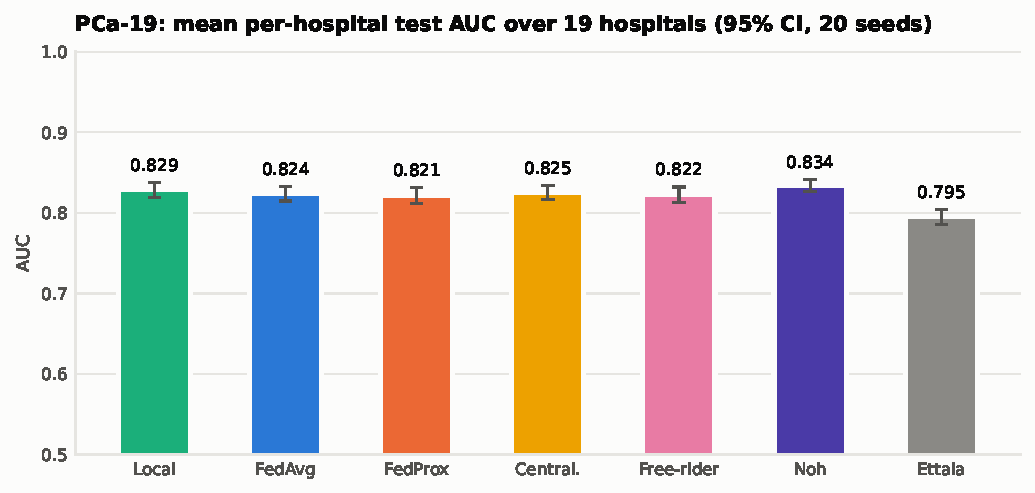
\includegraphics[width=\columnwidth]{figures/figure14_pca19_strategies.pdf}
\caption{PCa-19: mean per-hospital test AUC of each strategy over the 19 real hospitals (20 seeds, 95\% CI).}
\label{fig:pca19_strategies}
\end{figure}


\subsection{External Validation and Calibration}
\label{sec:p19_loco}
The base paper evaluates only within its hospital set. We add \emph{leave-one-country-out} validation: models are trained on seven countries and tested on all patients of the eighth (Table~\ref{tab:pca19_loco}); preprocessing statistics never include the held-out country. Treating the eight countries as independent external tests, federated training matches centralised training (FedAvg$-$CEN $=\pLocoAvgCen$) and the published Noh calculator (FedAvg$-$Noh $=\pLocoAvgNoh$). DP at $\varepsilon=5$ costs a small but significant $\pLocoDpFive$ AUC.

Discrimination transports across countries; calibration does not. Observed/expected ratios of the FedAvg model range from \pOeMin{} to \pOeMax{} across countries, reflecting different csPCa prevalence (12--47\%). DP adds a second, previously unreported effect: it makes predictions more extreme. The mean calibration slope is $\pSlopeNoDP$ without DP but $\pSlopeDpFive$ at $\varepsilon=5$ and $\pSlopeDpOne$ at $\varepsilon=1$; the last two intervals exclude 1. A simple fix, and one that is already common clinical practice (risk calculators are routinely recalibrated to the local population before use, and some publications omit the intercept for this reason), is \emph{local recalibration} on 20\% of a new country's patients (Table~\ref{tab:pca19_recal}, Fig.~\ref{fig:pca19_recal}). Re-estimating only the intercept reduces $|\log \mathrm{O/E}|$ from \pRecalOeRaw{} to \pRecalOeInt{} (paired difference $\pRecalOeDiff$). Re-estimating intercept and slope restores the DP model's slope from \pRecalSlopeDpRaw{} to \pRecalSlopeDpLog{}. Neither step changes the AUC, and both use only a few dozen to a few hundred local patients. Decision-curve analysis (Fig.~\ref{fig:pca19_dca}) shows positive net benefit over biopsying all men for every federated model at thresholds of 10--40\%.

\begin{table*}[t]
\caption{Leave-one-country-out external validation on PCa-19: train on the other seven countries, test on all patients of the held-out country (mean of 20 seeds). O/E = observed/expected events; slope = calibration slope (ideal 1).}
\centering\small
\begin{tabular}{lrrccccccc}
\toprule
& & & \multicolumn{3}{c}{FedAvg} & \multicolumn{2}{c}{FedProx + DP ($\varepsilon=5$)} & \multicolumn{2}{c}{Noh (published)} \\
Country & $n$ & csPCa\% & AUC & O/E & slope & AUC & slope & AUC & O/E \\
\midrule
China & 842 & 31 & 0.872 & 0.78 & 1.08 & 0.851 & 0.81 & 0.874 & 0.97 \\
Germany & 925 & 43 & 0.842 & 1.01 & 1.07 & 0.844 & 0.79 & 0.833 & 1.12 \\
Italy & 218 & 12 & 0.821 & 0.47 & 0.89 & 0.819 & 0.67 & 0.825 & 0.54 \\
Netherlands & 266 & 26 & 0.904 & 0.83 & 1.30 & 0.877 & 1.00 & 0.934 & 1.03 \\
South Korea & 996 & 33 & 0.896 & 0.83 & 1.45 & 0.890 & 1.01 & 0.886 & 1.00 \\
Spain & 1640 & 46 & 0.825 & 1.24 & 0.93 & 0.820 & 0.72 & 0.819 & 1.31 \\
USA & 590 & 47 & 0.783 & 1.30 & 0.86 & 0.776 & 0.65 & 0.765 & 1.55 \\
United Kingdom & 133 & 29 & 0.905 & 0.78 & 1.10 & 0.903 & 0.83 & 0.907 & 0.88 \\
\bottomrule
\end{tabular}
\label{tab:pca19_loco}
\end{table*}



\begin{figure}[!t]
\centering
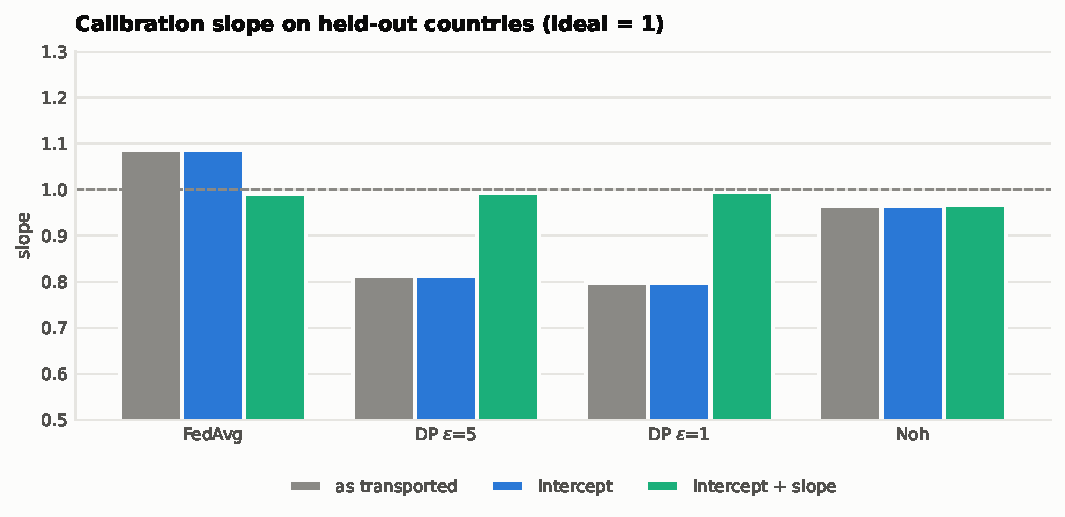
\includegraphics[width=\columnwidth]{figures/figure17_pca19_recalibration.pdf}
\caption{Calibration slope on held-out countries before and after local recalibration on 20\% of the country's patients.}
\label{fig:pca19_recal}
\end{figure}

\begin{figure}[!t]
\centering
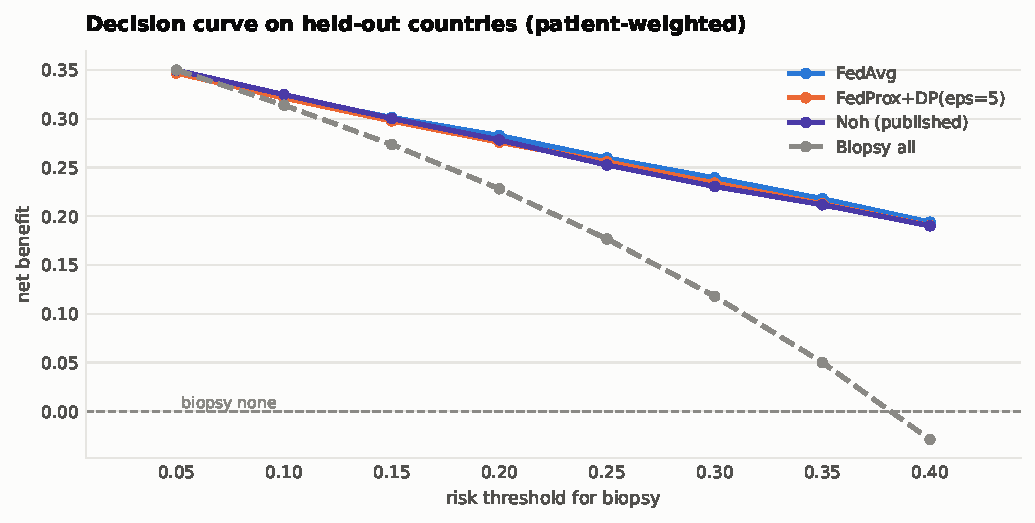
\includegraphics[width=\columnwidth]{figures/figure16_pca19_dca.pdf}
\caption{Decision curves on held-out countries (patient-weighted over the eight leave-one-country-out folds).}
\label{fig:pca19_dca}
\end{figure}




\subsection{Privacy and Drift on Real Hospitals}
Table~\ref{tab:pca19_privacy} and Fig.~\ref{fig:pca19_privacy} report the privacy--utility grid on the real hospitals. With \pNineN{} patients, privacy is almost free. Even at $\varepsilon=0.5$ ($\sigma=\pSigmaHalf$) the mean per-hospital AUC changes by only $\pDpLossHalf$. This small cost should not be generalised: it holds for a seven-parameter, regularised logistic model trained on about 4{,}500 patients. The effect of a given $\varepsilon$ depends strongly on the model and the amount of data. For the non-convex federated MLP of the main paper the DP releases are far noisier than for logistic regression (Section~\ref{sec:p19_mlp}); for simple logistic models even very different $\varepsilon$ can give nearly the same result. FedProx reduces client drift by \pDriftRed\%, and DP noise inflates drift about tenfold at $\varepsilon=0.5$. At every privacy level, FedProx equals FedAvg with half the learning rate (largest mean difference \pProxHalfMax{} AUC). FedProx's benefit here is therefore a step-size effect.



\begin{figure}[!t]
\centering
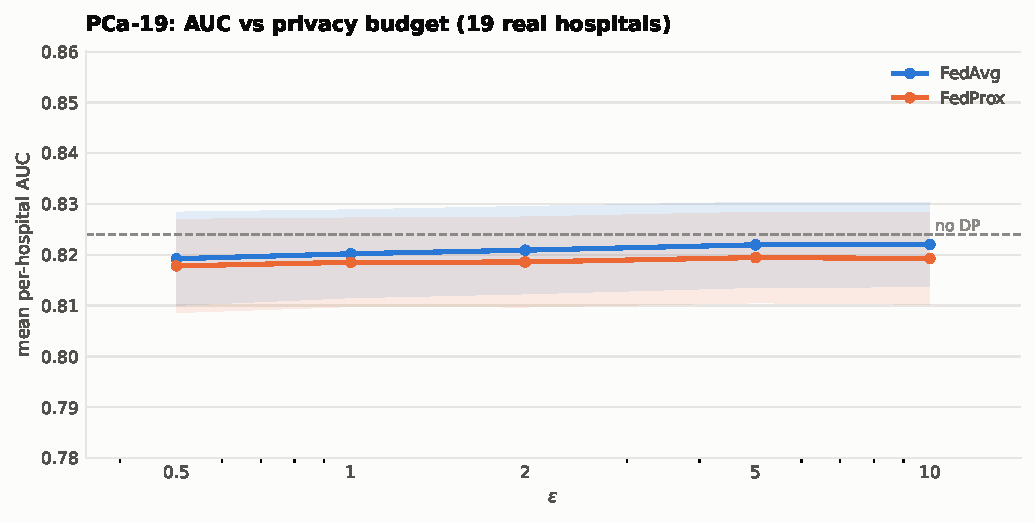
\includegraphics[width=\columnwidth]{figures/figure15_pca19_privacy.pdf}
\caption{PCa-19: mean per-hospital AUC vs privacy budget (20 seeds, 95\% CI); dashed line = no DP.}
\label{fig:pca19_privacy}
\end{figure}

\subsection{Stronger Baselines}
\label{sec:p19_baselines}
Table~\ref{tab:baselines} adds SCAFFOLD \cite{Karimireddy2020Scaffold}, FedAdam \cite{Reddi2021FedOpt}, a federated one-hidden-layer MLP, a converged FedAvg (400 instead of 100 local steps) and centralised non-linear references (histogram gradient boosting in the style of LightGBM \cite{Ke2017LightGBM}, random forest, MLP). FedNova \cite{Wang2020FedNova} normalises by the number of local steps and therefore equals FedAvg here, where every hospital runs the same number of steps. Hyper-parameters of the new baselines were tuned on four splits disjoint from the 20 evaluation splits. All federated variants lie within 0.006 AUC of FedAvg within hospitals: FedAdam $\blDAdam$, federated MLP $\blDMLP$, converged FedAvg $\blDLong$. SCAFFOLD removes \blScafDrift\% of client drift (FedProx: \blProxDrift\%) without changing AUC ($\blDScaf$). Under DP at $\varepsilon=1$ no variant improves on FedAvg (SCAFFOLD $\blDpScaf$, FedAdam $\blDpAdam$). Pooled non-linear models gain a little within the training hospitals (gradient boosting $\blDGB$) but not on unseen countries (gradient boosting $\blLGB$, federated MLP $\blLMLP$), where they are also less well calibrated. With four pre-biopsy variables, the information in the data, not the model class or the federated optimiser, sets the ceiling; logistic regression is adequate and the best calibrated.

\begin{table*}[t]
\caption{Stronger baselines on PCa-19 (20 held-out seeds). Within-hospital: mean per-hospital test AUC over 19 hospitals. Leave-one-country-out: mean AUC over the 8 held-out countries and mean calibration slope; differences vs FedAvg are paired over countries ($n=8$). Last column: federated variants trained with DP at $\varepsilon=1$. FedNova equals FedAvg here (identical local steps at every hospital).}
\centering\small
\begin{tabular}{lcccccc}
\toprule
& \multicolumn{2}{c}{Within hospital} & \multicolumn{3}{c}{Leave-one-country-out} & DP \\
Model & AUC & $-$FedAvg [95\% CI] & AUC & $-$FedAvg [95\% CI] & Slope & $\varepsilon=1$ \\
\midrule
FedAvg & 0.816 & -- & 0.856 & -- & 1.08 & 0.811 \\
FedAvg (400 steps) & 0.818 & $+0.002\ [+0.001, +0.003]$ & 0.860 & $+0.004\ [\ensuremath{-}0.001, +0.009]$ & 1.02 & -- \\
FedProx & 0.811 & $-0.005\ [\ensuremath{-}0.008, \ensuremath{-}0.002]$ & 0.853 & $-0.003\ [\ensuremath{-}0.007, +0.000]$ & 1.12 & 0.809 \\
SCAFFOLD & 0.816 & $-0.000\ [\ensuremath{-}0.001, +0.000]$ & 0.856 & $+0.000\ [\ensuremath{-}0.001, +0.001]$ & 1.08 & 0.811 \\
FedAdam & 0.818 & $+0.002\ [+0.000, +0.005]$ & 0.861 & $+0.005\ [\ensuremath{-}0.003, +0.012]$ & 1.07 & 0.807 \\
Federated MLP & 0.821 & $+0.005\ [+0.001, +0.009]$ & 0.861 & $+0.005\ [\ensuremath{-}0.000, +0.010]$ & 0.92 & -- \\
\midrule
Central LR & 0.819 & $+0.003\ [+0.000, +0.005]$ & 0.860 & $+0.005\ [\ensuremath{-}0.002, +0.011]$ & 1.02 & -- \\
Central gradient boosting & 0.824 & $+0.009\ [+0.004, +0.014]$ & 0.853 & $-0.003\ [\ensuremath{-}0.011, +0.004]$ & 0.91 & -- \\
Central random forest & 0.820 & $+0.004\ [\ensuremath{-}0.002, +0.011]$ & 0.850 & $-0.006\ [\ensuremath{-}0.013, +0.001]$ & 0.95 & -- \\
Central MLP & 0.828 & $+0.012\ [+0.007, +0.017]$ & 0.861 & $+0.005\ [\ensuremath{-}0.001, +0.012]$ & 1.00 & -- \\
\bottomrule
\end{tabular}
\label{tab:baselines}
\end{table*}


\subsection{Sensitivity to Training Length}
Our default of $T=20$ rounds and $E=5$ local epochs (100 gradient steps) was fixed in an earlier phase of the project and keeps the DP noise per step moderate. On PCa-19 it is slightly under-converged for some splits. Repeating the strategy comparison with 400 steps leaves every conclusion unchanged: FL$-$LOC $=\cvgFLminusLOC$, FR$-$FL $=\cvgFRminusFL$, CEN$-$FL $=\cvgCENminusFL$, and the published Noh calculator remains ahead on the hospital-averaged AUC (FL$-$Noh $=\cvgFLminusNoh$) but behind on the patient-weighted AUC (\cvgWFL{} vs \cvgWNoh{}).

\subsection{Personalisation}
Proximal fine-tuning helps exactly where expected. For the \pNSmall{} hospitals with fewer than 100 patients it improves on the global FedProx model by $\pPflSmall$ AUC, and over all hospitals by $\pPflAll$. For large hospitals ($\geq 400$ patients) it brings no gain ($\pPflLarge$), and these hospitals are slightly better served by their own local model (FedProx$-$Local $=\pPflLargeLoc$).

\subsection{Subsampled Privacy Accounting}
\label{sec:p19_subsampling}
Our main experiments use full-batch updates ($q=1$), for which no privacy amplification can be claimed. Table~\ref{tab:subsampling} replaces them by Poisson-subsampled DP-SGD with sampled-Gaussian RDP accounting. Amplification lowers the noise multiplier needed for $\varepsilon=1$ from \ssSigFull{} (full batch) to \ssSigThree{} ($q=0.3$) and \ssSigOne{} ($q=0.1$). It does not, however, improve utility on held-out splits. On PCa-19 the AUC difference to full batch at $\varepsilon=1$ is $\ssPThreeOne$ for $q=0.3$. Smaller expected batches and more steps offset the lower noise multiplier (learning rates for $q<1$ were tuned on separate splits; a modest gain seen there did not replicate). The conservative full-batch accounting is therefore not what limits utility in this setting. Calibration slopes under DP are equally below 1 with and without subsampling.




\subsection{Retraining-Based Valuation under DP: Full Results}
\label{sec:retrain_full}
We first follow the standard approach and retrain every coalition with DP at a per-run $\varepsilon$ (its real privacy cost is examined in Section~\ref{sec:p19_osa}). We computed exact Shapley values over the ten largest hospitals (1{,}023 coalitions) and, for all 19 hospitals, stratified-sampling Shapley values. Sampling is stratified by coalition size, and the two largest strata (a hospital alone, and leave-one-out) are computed exactly. This needs \pShNineCoal{} coalitions per seed instead of $2^{19}$, and a validation check shows it agrees with exact Shapley to within 0.003 AUC, where plain permutation sampling with 400 permutations errs by 0.014. Rankings are fairly robust under weak privacy but not under strong privacy (Table~\ref{tab:pca19_shapley}). With ten hospitals, the Spearman correlation with the no-DP ranking is \pShRhoTen{} at $\varepsilon=10$, \pShRhoTwo{} at $\varepsilon=2$, \pShRhoOne{} at $\varepsilon=1$ and \pShRhoHalf{} at $\varepsilon=0.5$, while the AUC changes by less than 0.01 over the same range. Because the hospitals' contributions are close together (Shapley values \pShPhiMin--\pShPhiMax{} AUC), the identity of the top contributor is fragile even under weak privacy: it keeps its place in \pShTSTen{} of runs at $\varepsilon=10$ and \pShTSHalf{} at $\varepsilon=0.5$. With all 19 hospitals the correlation is \pShNineRhoFive{} at $\varepsilon=5$ and \pShNineRhoOne{} at $\varepsilon=1$, and the top contributor keeps its place in \pShNineTSFive{} and \pShNineTSOne{} of runs. Leave-one-out values are near zero for every hospital, so leave-one-out cannot separate contributors (Spearman with Shapley \pShLooRho). The instability of contribution rankings under DP therefore appears on real hospitals at strong privacy levels where accuracy is still unaffected, and for the top-ranked position at every privacy level.




\subsection{Membership Inference}
The confidence-threshold attack is at chance for every model (AUC \pMiaNoDP{} without DP), while it reaches \pMiaCtl{} on an over-fitted control model. A seven-parameter model trained on about 4{,}500 patients does not memorise individuals, so the empirical audit again cannot show a DP benefit; DP remains a guarantee against all attacks, including stronger ones not tested here.


\section{Detailed PCa-19 Tables}
This section collects the detailed tables of the PCa-19 evaluation referred to in the main text.

\begin{table}[t]
\caption{PCa-19: the base paper's 19-hospital pre-biopsy cohort (5{,}610 men). csPCa = ISUP grade group $\geq 2$ at biopsy; medians of age (years), PSA (ng/mL) and prostate volume (mL); PI-RADS $\geq 4$ in \%.}
\centering\scriptsize
\setlength{\tabcolsep}{3pt}
\begin{tabular}{llrrrrrr}
\toprule
Hosp. & Country & $n$ & csPCa\% & Age & PSA & Vol. & PI-RADS$\geq$4 \\
\midrule
de1 & Germany & 763 & 43 & 65 & 8.0 & 47 & 74 \\
es7 & Spain & 711 & 50 & 67 & 7.6 & 53 & 55 \\
kr2 & South Korea & 590 & 38 & 68 & 7.0 & 42 & 72 \\
ch2 & China & 530 & 33 & 67 & 10.3 & 41 & 42 \\
kr1 & South Korea & 406 & 25 & 64 & 6.8 & 36 & 28 \\
es6 & Spain & 346 & 43 & 69 & 7.6 & 52 & 78 \\
ch1 & China & 312 & 27 & 66 & 9.7 & 45 & 43 \\
us2 & USA & 310 & 48 & 65 & 7.3 & 46 & 82 \\
us1 & USA & 280 & 45 & 62 & 5.5 & 45 & 62 \\
nl & Netherlands & 266 & 26 & 67 & 11.1 & 56 & 36 \\
it & Italy & 218 & 12 & 65 & 8.0 & 54 & 38 \\
es4 & Spain & 200 & 34 & 69 & 7.6 & 55 & 56 \\
es5 & Spain & 200 & 47 & 70 & 10.6 & 56 & 80 \\
de2 & Germany & 162 & 47 & 65 & 6.5 & 40 & 70 \\
gb & United Kingdom & 133 & 29 & 64 & 7.6 & 45 & 48 \\
es1 & Spain & 79 & 42 & 69 & 6.3 & 61 & 97 \\
es8 & Spain & 58 & 38 & 70 & 6.5 & 56 & 81 \\
es3 & Spain & 30 & 60 & 69 & 9.0 & 50 & 97 \\
es2 & Spain & 16 & 38 & 64 & 277.0 & 81 & 69 \\
\bottomrule
\end{tabular}
\label{tab:pca19_cohort}
\end{table}

\begin{table*}[t]
\caption{Privacy and drift on the 19 real hospitals (mean per-hospital test AUC, 20 seeds). The last two AUC columns are paired differences with 95\% CI; drift = mean $\|w_k-w^{t-1}\|$.}
\centering\small
\begin{tabular}{lccccccc}
\toprule
$\varepsilon$ & $\sigma$ & FedAvg & FedProx & FedAvg ($\eta/2$) & FedAvg $-$ no DP & FedProx $-$ FedAvg($\eta/2$) & Drift Avg / Prox \\
\midrule
no DP & -- & 0.824 & 0.821 & 0.821 & $--$ & $+0.000\ [\ensuremath{-}0.001, +0.002]$ & 0.33 / 0.23 \\
10 & 5.7 & 0.822 & 0.819 & 0.819 & $-0.002\ [\ensuremath{-}0.007, +0.003]$ & $+0.000\ [\ensuremath{-}0.001, +0.002]$ & 0.35 / 0.24 \\
5 & 10.5 & 0.822 & 0.819 & 0.819 & $-0.002\ [\ensuremath{-}0.007, +0.003]$ & $+0.000\ [\ensuremath{-}0.001, +0.002]$ & 0.48 / 0.33 \\
2 & 25.0 & 0.821 & 0.819 & 0.820 & $-0.003\ [\ensuremath{-}0.007, +0.001]$ & $-0.001\ [\ensuremath{-}0.003, +0.001]$ & 0.91 / 0.61 \\
1 & 49.0 & 0.820 & 0.819 & 0.819 & $-0.004\ [\ensuremath{-}0.008, +0.001]$ & $-0.001\ [\ensuremath{-}0.003, +0.002]$ & 1.69 / 1.13 \\
0.5 & 97.0 & 0.819 & 0.818 & 0.819 & $-0.005\ [\ensuremath{-}0.011, +0.001]$ & $-0.001\ [\ensuremath{-}0.003, +0.001]$ & 3.30 / 2.19 \\
\bottomrule
\end{tabular}
\label{tab:pca19_privacy}
\end{table*}

\begin{table}[t]
\caption{Local recalibration on 20\% of each held-out country, evaluated on the other 80\% (mean over 8 countries and 20 seeds). $|\log$ O/E$|$ = 0 and slope = 1 are ideal; DP rows are FedProx + DP.}
\centering\scriptsize
\setlength{\tabcolsep}{4pt}
\begin{tabular}{llccc}
\toprule
Model & Recalibration & $|\log$ O/E$|$ & Slope & Brier \\
\midrule
FedAvg & none & 0.263 & 1.09 & 0.145 \\
 & intercept & 0.071 & 1.09 & 0.136 \\
 & int.\,+\,slope & 0.074 & 0.99 & 0.138 \\
\midrule
DP $\varepsilon=5$ & none & 0.260 & 0.81 & 0.150 \\
 & intercept & 0.080 & 0.81 & 0.140 \\
 & int.\,+\,slope & 0.074 & 0.99 & 0.140 \\
\midrule
DP $\varepsilon=1$ & none & 0.263 & 0.80 & 0.151 \\
 & intercept & 0.081 & 0.80 & 0.140 \\
 & int.\,+\,slope & 0.074 & 1.00 & 0.140 \\
\midrule
Noh & none & 0.205 & 0.97 & 0.144 \\
 & intercept & 0.075 & 0.97 & 0.137 \\
 & int.\,+\,slope & 0.077 & 0.97 & 0.138 \\
\bottomrule
\end{tabular}
\label{tab:pca19_recal}
\end{table}

\begin{table}[t]
\caption{Stability of Shapley contribution rankings under DP on the real PCa-19 hospitals (20 seeds). $\rho$ = Spearman correlation with the no-DP ranking; Rank rev.\ = share of hospital pairs whose order flips relative to the no-DP ranking; TS = probability that the no-DP top contributor stays first.}
\centering\scriptsize
\begin{tabular}{lcccc}
\toprule
Hospitals & $\varepsilon$ & $\rho$ [95\% CI] & Rank rev. & TS \\
\midrule
10 (exact) & 10 & $0.94\ [0.93, 0.95]$ & 0.44 & 0.75 \\
10 (exact) & 5 & $0.94\ [0.92, 0.95]$ & 0.45 & 0.75 \\
10 (exact) & 2 & $0.91\ [0.90, 0.93]$ & 0.57 & 0.80 \\
10 (exact) & 1 & $0.85\ [0.80, 0.90]$ & 0.64 & 0.70 \\
10 (exact) & 0.5 & $0.64\ [0.56, 0.71]$ & 0.79 & 0.40 \\
19 (stratified) & 5 & $0.90\ [0.87, 0.93]$ & 0.80 & 0.45 \\
19 (stratified) & 1 & $0.76\ [0.71, 0.80]$ & 0.84 & 0.45 \\
\bottomrule
\end{tabular}
\label{tab:pca19_shapley}
\end{table}

\begin{table}[t]
\caption{Poisson subsampling with sampled-Gaussian RDP accounting (FedProx, 20 held-out seeds). $\sigma$ = noise multiplier needed for the stated $\varepsilon$ over the given number of local steps; PCa-19: mean per-hospital AUC (difference to full batch in brackets) and calibration slope.}
\centering\scriptsize
\setlength{\tabcolsep}{3pt}
\begin{tabular}{lccccc}
\toprule
Sampling & $\varepsilon$ & $\sigma$ & Steps & AUC & Slope \\
\midrule
full batch (q=1) & no DP & -- & 100 & 0.811 & 1.08 \\
full batch (q=1) & 10 & 5.7 & 100 & 0.811 & 0.78 \\
full batch (q=1) & 5 & 10.5 & 100 & 0.810 & 0.78 \\
full batch (q=1) & 2 & 25.0 & 100 & 0.810 & 0.77 \\
full batch (q=1) & 1 & 49.0 & 100 & 0.809 & 0.76 \\
full batch (q=1) & 0.5 & 97.0 & 100 & 0.806 & 0.72 \\
\midrule
q=0.3 & no DP & -- & 300 & 0.810 ($-0.001$) & 1.09 \\
q=0.3 & 10 & 3.1 & 300 & 0.810 ($-0.001$) & 0.79 \\
q=0.3 & 5 & 5.6 & 300 & 0.810 ($+0.000$) & 0.79 \\
q=0.3 & 2 & 13.1 & 300 & 0.809 ($-0.001$) & 0.79 \\
q=0.3 & 1 & 25.6 & 300 & 0.810 ($+0.001$) & 0.78 \\
q=0.3 & 0.5 & 50.5 & 300 & 0.809 ($+0.003$) & 0.75 \\
\midrule
q=0.1 & no DP & -- & 1000 & 0.810 ($-0.001$) & 1.08 \\
q=0.1 & 10 & 2.0 & 1000 & 0.810 ($-0.001$) & 0.79 \\
q=0.1 & 5 & 3.5 & 1000 & 0.809 ($-0.000$) & 0.79 \\
q=0.1 & 2 & 8.0 & 1000 & 0.810 ($-0.000$) & 0.78 \\
q=0.1 & 1 & 15.6 & 1000 & 0.809 ($+0.000$) & 0.77 \\
q=0.1 & 0.5 & 30.8 & 1000 & 0.807 ($+0.000$) & 0.73 \\
\bottomrule
\end{tabular}
\label{tab:subsampling}
\end{table}

\begin{table}[t]
\caption{OSA-Shapley robustness on PCa-19 (ten hospitals, 20 held-out seeds). Top: Spearman $\rho$ with the exact non-private ranking. Bottom: share of splits in which a hospital with random training labels (es6) is ranked last (no-DP retraining Shapley: 100\%).}
\centering\scriptsize
\begin{tabular}{lcc}
\toprule
Setting & $\varepsilon=2$ & $\varepsilon=1$ \\
\midrule
Local steps = 10 & 0.84 & 0.81 \\
Local steps = 30 (chosen) & 0.89 & 0.80 \\
Local steps = 60 & 0.90 & 0.72 \\
Reference set 25\% of hospital test data & 0.77 & 0.67 \\
Reference set 50\% of hospital test data & 0.87 & 0.77 \\
\midrule
\multicolumn{3}{l}{\emph{Useless hospital ranked last}} \\
OSA (cost $\varepsilon$) & 100\% & 95\% \\
MR (cost $\varepsilon$) & 70\% & 80\% \\
OR (cost $\varepsilon$) & 100\% & 100\% \\
Retraining, budget-matched (cost $\varepsilon$) & 60\% & 45\% \\
Retraining, per run (true $\varepsilon$ 85 and 33) & 100\% & 100\% \\
\bottomrule
\end{tabular}
\label{tab:osa_robust}
\end{table}

\begin{figure}[!t]
\centering
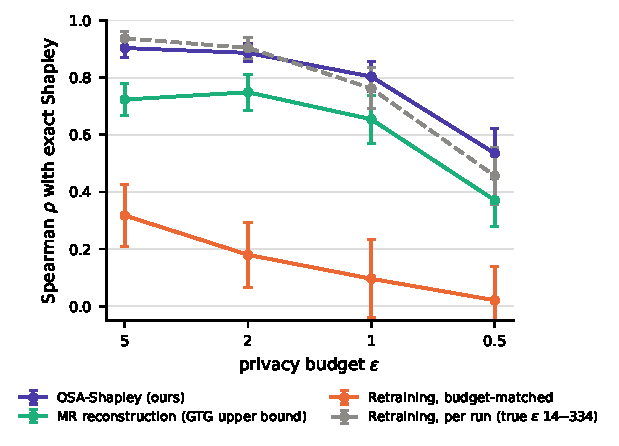
\includegraphics[width=\columnwidth]{figures/figure19_osa_valuation.pdf}
\caption{Agreement of each valuation with the exact non-private Shapley ranking of the ten largest PCa-19 hospitals (20 held-out splits, 95\% CI). OSA-Shapley, MR reconstruction and budget-matched retraining all cost the stated $\varepsilon$; per-run retraining costs the composed $\varepsilon$ of Table~\ref{tab:osa}.}
\label{fig:osa}
\end{figure}
\begin{table*}[t]
\caption{Contribution valuation under DP on the ten largest PCa-19 hospitals (20 held-out seeds). Agreement with the exact non-private Shapley ranking (Spearman $\rho$) and probability that the true top contributor is ranked first (TS). \emph{Per-run}: every coalition retrained at the stated $\varepsilon$, whose true cost for each hospital is the composed $\varepsilon$ in column 2. \emph{Budget-matched}: retraining with noise calibrated so that the total cost is the stated $\varepsilon$. OSA-Shapley costs the stated $\varepsilon$ once.}
\centering\small
\begin{tabular}{lccccccc}
\toprule
 & True $\varepsilon$ of & \multicolumn{3}{c}{Spearman $\rho$ with exact Shapley} & \multicolumn{3}{c}{TS} \\
$\varepsilon$ & per-run retraining & per-run & budget-matched & OSA & per-run & budget-matched & OSA \\
\midrule
10 & 988 & 0.94 & 0.47 & \textbf{0.90} & 0.75 & 0.45 & \textbf{0.60} \\
5 & 334 & 0.94 & 0.32 & \textbf{0.90} & 0.70 & 0.35 & \textbf{0.60} \\
2 & 85 & 0.90 & 0.18 & \textbf{0.89} & 0.65 & 0.10 & \textbf{0.55} \\
1 & 33 & 0.76 & 0.10 & \textbf{0.80} & 0.55 & 0.10 & \textbf{0.40} \\
0.5 & 14 & 0.46 & 0.02 & \textbf{0.54} & 0.50 & 0.05 & \textbf{0.35} \\
\bottomrule
\end{tabular}
\label{tab:osa}
\end{table*}

\begin{table}[t]
\caption{Valuation with a non-convex model: a one-hidden-layer MLP (16 tanh units, weight decay $10^{\ensuremath{-}3}$) trained by FedAvg. Spearman $\rho$ with the exact non-private retraining Shapley ranking of the ten largest PCa-19 hospitals (20 held-out splits; budget-matched retraining on 5 of them). OSA-ens.: coalition prediction = size-weighted average of the members' log-odds; OSA-par.: size-weighted parameter average from a shared initialisation; MR: exact multi-round reconstruction from one DP FedAvg-MLP run. All columns cost the stated $\varepsilon$.}
\centering\scriptsize
\setlength{\tabcolsep}{4pt}
\begin{tabular}{lccccc}
\toprule
$\varepsilon$ & OSA-ens. & OSA-par. & MR & OSA-ens.$-$MR & Budget-m. \\
\midrule
none & 0.91 & 0.67 & 0.78 & $+0.13\ [+0.07, +0.19]$ & -- \\
5 & 0.68 & 0.52 & 0.82 & $-0.14\ [\ensuremath{-}0.19, \ensuremath{-}0.09]$ & -- \\
2 & 0.65 & 0.65 & 0.82 & $-0.17\ [\ensuremath{-}0.25, \ensuremath{-}0.09]$ & 0.16 \\
1 & 0.60 & 0.60 & 0.78 & $-0.18\ [\ensuremath{-}0.29, \ensuremath{-}0.07]$ & 0.05 \\
0.5 & 0.42 & 0.44 & 0.74 & $-0.32\ [\ensuremath{-}0.46, \ensuremath{-}0.18]$ & -- \\
\bottomrule
\end{tabular}
\label{tab:osa_mlp}
\end{table}

\begin{table*}[t]
\caption{Valuations that cost the privacy budget once (Spearman $\rho$ with the exact non-private retraining Shapley ranking). OSA: one DP model per hospital. MR: exact multi-round reconstruction from one DP-FedAvg run (GTG-Shapley is its truncated Monte-Carlo approximation). OR: one-round reconstruction from the same run. All three are post-processing of releases that already cost $\varepsilon$. OSA$-$MR: paired difference with 95\% CI. Both groups are real PCa-19 hospitals, 20 held-out splits; no hospital is simulated or partitioned.}
\centering\small
\begin{tabular}{lcccccccc}
\toprule
 & \multicolumn{4}{c}{Ten largest hospitals (266--763 patients)} & \multicolumn{4}{c}{Ten smallest hospitals (16--266 patients)} \\
\cmidrule(lr){2-5}\cmidrule(lr){6-9}
$\varepsilon$ & OSA & MR & OR & OSA$-$MR & OSA & MR & OR & OSA$-$MR \\
\midrule
none & \textbf{0.96} & 0.74 & 0.42 & $+0.22\ [+0.18, +0.27]$ & \textbf{0.95} & 0.86 & 0.79 & $+0.10\ [+0.05, +0.14]$ \\
5 & \textbf{0.90} & 0.72 & 0.53 & $+0.18\ [+0.14, +0.22]$ & \textbf{0.85} & 0.83 & 0.81 & $+0.03\ [\ensuremath{-}0.00, +0.06]$ \\
2 & \textbf{0.89} & 0.75 & 0.51 & $+0.14\ [+0.08, +0.19]$ & \textbf{0.79} & 0.78 & 0.74 & $+0.00\ [\ensuremath{-}0.06, +0.06]$ \\
1 & \textbf{0.80} & 0.65 & 0.50 & $+0.15\ [+0.03, +0.26]$ & \textbf{0.68} & 0.74 & 0.59 & $-0.06\ [\ensuremath{-}0.15, +0.03]$ \\
0.5 & \textbf{0.54} & 0.37 & 0.39 & $+0.16\ [+0.04, +0.29]$ & -- & -- & -- & -- \\
\bottomrule
\end{tabular}
\label{tab:osa_post}
\end{table*}


\section{Pre-Registered Test of the Decision Rule}
\label{sec:prereg}
\begin{table*}[t]
\caption{Evidence behind the decision rule, from two real federations. $p$: model parameters; $\nu$: median training patients per hospital divided by $\sqrt p$, which sets the signal-to-noise ratio of one DP release (Proposition~3). $\rho$: Spearman correlation with the exact non-private retraining Shapley ranking (20 held-out splits). OSA$-$MR: paired difference with 95\% CI at $\varepsilon=2$. Size: agreement of hospital size with the same ranking.}
\centering\small
\begin{tabular}{llrrrcccccl}
\toprule
 & & & & & OSA & OSA & MR & & & \\
Federation & Model & $K$ & $p$ & $\nu$ & no DP & $\varepsilon=2$ & $\varepsilon=2$ & OSA$-$MR & Size & Best at $\varepsilon=2$ \\
\midrule
PCa-19, 10 largest & logistic & 10 & 7 & 114 & 0.96 & 0.89 & 0.75 & $+0.14\ [+0.08, +0.19]$ & 0.08 & OSA \\
PCa-19, 10 smallest & logistic & 10 & 7 & 45 & 0.95 & 0.79 & 0.78 & $+0.00\ [\ensuremath{-}0.06, +0.06]$ & 0.74 & OSA, MR or size \\
Heart Disease, 4 & logistic & 4 & 21 & 43 & 0.92 & 0.15 & 0.45 & $-0.30\ [\ensuremath{-}0.59, \ensuremath{-}0.01]$ & \ensuremath{-}0.38 & MR \\
PCa-19, 10 largest & MLP & 10 & 129 & 26 & 0.91 & 0.65 & 0.82 & $-0.17\ [\ensuremath{-}0.25, \ensuremath{-}0.09]$ & -- & MR \\
\bottomrule
\end{tabular}
\label{tab:decision}
\end{table*}

The design and hypotheses below were written before the sweep was run and fixed by their SHA-256 hash (\texttt{results/preregistration\_nu\_sweep.md}, hash \texttt{3d5dfcdf\ldots68a1}, 17 Oct 2026, 08:19 UTC); a copy was saved on a second machine at the same time. The registration is internal (a hash, not a public registry such as OSF), and the protocol was written and run on the same day. Its timing therefore cannot be verified by third parties; future tests of the revised rule will be registered publicly (for example on OSF) before they are run. Hypotheses at $\varepsilon=2$: (H1) OSA$-$MR $>0$ for $\nu\ge100$; (H2) OSA$-$MR not positive for $\nu\le50$; (H3) OSA$-$MR increases with $\nu$; (H4) the sign change lies between $\nu=50$ and 100; (H5) both arms agree at matched $\nu$; (H6) at $\varepsilon=1$ the switch-over lies at higher $\nu$, or OSA$-$MR is lower in at least six of eight conditions. Outcome: H1, H3, H5 and H6 supported (H6 through the higher switch-over; OSA$-$MR was lower at $\varepsilon=1$ in \nsLowerCount{} of 8 conditions); H2 and H4 not supported. No condition, seed or setting was changed after the results were seen. Full results are in Table~\ref{tab:nu_sweep}.

\begin{table*}[t]
\caption{Pre-registered test of the decision rule on the ten largest PCa-19 hospitals (20 held-out splits). Arm A keeps a random fraction of every hospital's training patients; arm B adds uninformative features. In every condition the reference is the exact non-private retraining Shapley ranking of that condition. $\rho$: Spearman correlation with the reference; OSA$-$MR: paired difference with 95\% CI.}
\centering\small
\begin{tabular}{lrrcccccc}
\toprule
 & & & \multicolumn{3}{c}{$\varepsilon=2$} & \multicolumn{3}{c}{$\varepsilon=1$} \\
\cmidrule(lr){4-6}\cmidrule(lr){7-9}
Condition & $p$ & $\nu$ & OSA & MR & OSA$-$MR & OSA & MR & OSA$-$MR \\
\midrule
A: 100\% of patients & 7 & 113 & 0.89 & 0.75 & $+0.14\ [+0.08, +0.19]$ & 0.80 & 0.65 & $+0.15\ [+0.03, +0.26]$ \\
A: 60\% of patients & 7 & 68 & 0.80 & 0.72 & $+0.08\ [+0.00, +0.16]$ & 0.65 & 0.51 & $+0.14\ [+0.02, +0.26]$ \\
A: 40\% of patients & 7 & 45 & 0.74 & 0.55 & $+0.18\ [+0.08, +0.29]$ & 0.48 & 0.36 & $+0.12\ [\ensuremath{-}0.04, +0.27]$ \\
A: 25\% of patients & 7 & 28 & 0.58 & 0.46 & $+0.12\ [+0.00, +0.24]$ & 0.40 & 0.36 & $+0.04\ [\ensuremath{-}0.07, +0.16]$ \\
A: 15\% of patients & 7 & 17 & 0.52 & 0.61 & $-0.09\ [\ensuremath{-}0.20, +0.03]$ & 0.35 & 0.53 & $-0.18\ [\ensuremath{-}0.32, \ensuremath{-}0.03]$ \\
B: +21 features & 28 & 57 & 0.78 & 0.71 & $+0.07\ [\ensuremath{-}0.03, +0.18]$ & 0.66 & 0.54 & $+0.13\ [+0.01, +0.24]$ \\
B: +50 features & 57 & 40 & 0.75 & 0.70 & $+0.05\ [\ensuremath{-}0.02, +0.12]$ & 0.64 & 0.62 & $+0.01\ [\ensuremath{-}0.08, +0.10]$ \\
B: +100 features & 107 & 29 & 0.75 & 0.71 & $+0.05\ [\ensuremath{-}0.02, +0.11]$ & 0.60 & 0.68 & $-0.07\ [\ensuremath{-}0.15, +0.00]$ \\
\bottomrule
\end{tabular}
\label{tab:nu_sweep}
\end{table*}


\section{Claims and Computed Verdicts}
Table~\ref{tab:hyp_summary} lists every claim of the study with the evidence and the verdict computed from the result files.
\begin{table*}[t]
\caption{Claim--evidence summary. Verdicts are computed from the result files: `supported' only if the 95\% CI of the paired difference over seeds excludes 0 in the claimed direction; the pre-registered rows are scored by the criteria fixed in advance (Section~\ref{sec:prereg}).}
\centering\scriptsize
\begin{tabular}{p{1.4cm}p{4.2cm}p{8.6cm}p{1.5cm}}
\toprule
Area & Claim & Evidence (mean [95\% CI]) & Verdict \\
\midrule
PCa-19 (19 hospitals) & Joining FL gives hospitals a significant average local gain & FL - LOC (mean per-hospital AUC) = \ensuremath{-}0.005 {[}-0.015, +0.006{]} & not significant \\
PCa-19 (19 hospitals) & Free-riders get (almost) the same model as participants & FR - FL = \ensuremath{-}0.002 {[}-0.002, \ensuremath{-}0.001{]} & supported \\
PCa-19 (19 hospitals) & Federated training matches pooled training & CEN - FL = +0.002 {[}-0.001, +0.004{]} & supported \\
PCa-19 (19 hospitals) & FL beats the published Noh calculator (hospital-averaged AUC) & FL - Noh = \ensuremath{-}0.010 {[}-0.016, \ensuremath{-}0.005{]}; patient-weighted FL 0.856 vs Noh 0.850 & opposite \\
PCa-19 (19 hospitals) & Our re-implementation reproduces the base paper's code exactly & noh: max $|$difference$|$ 1.2e-14 over 5x19 cells (50 repeats); ettala: max $|$difference$|$ 7.8e-15 over 5x19 cells (50 repeats) & supported \\
PCa-19 (19 hospitals) & Federated model transports to unseen countries as well as pooled training & leave-one-country-out, FedAvg - centralised = \ensuremath{-}0.000 {[}-0.001, +0.001{]} (8 countries) & supported \\
PCa-19 (19 hospitals) & DP lowers the calibration slope (predictions more extreme) on held-out countries & slope at $\varepsilon$=5 = 0.81 {[}0.70, 0.92{]} over 8 countries (no DP 1.12) & supported \\
PCa-19 (19 hospitals) & Local recalibration (20\% of a new country) fixes calibration-in-the-large & $|$log O/E$|$ recalibrated - transported = \ensuremath{-}0.193 {[}-0.347, \ensuremath{-}0.038{]} & supported \\
PCa-19 (19 hospitals) & Strong privacy ($\varepsilon$ = 0.5) costs $<$ 0.02 AUC at this scale & FedAvg($\varepsilon$=0.5) - no DP = \ensuremath{-}0.005 {[}-0.011, +0.001{]} & supported \\
PCa-19 (19 hospitals) & FedProx's effect equals halving FedAvg's learning rate & largest $|$FedProx - FedAvg(lr/2)$|$ over 6 privacy levels = 0.0009 AUC; drift reduction 30.8\% & explained by step size \\
PCa-19 (19 hospitals) & Personalisation helps small hospitals ($<$ 100 patients) & PFL - FedProx = +0.039 {[}+0.013, +0.065{]} & supported \\
PCa-19 (19 hospitals) & DP noise destabilises Shapley rankings of real hospitals & 10 hospitals: Spearman 0.94 ($\varepsilon$=10) $\rightarrow$ 0.64 ($\varepsilon$=0.5) & supported \\
PCa-19 (19 hospitals) & OSA-Shapley beats retraining at the same real privacy cost ($\varepsilon$ = 2) & Spearman with exact Shapley: OSA - budget-matched retraining = +0.71 {[}+0.58, +0.84{]} & supported \\
PCa-19 (19 hospitals) & OSA-Shapley is not significantly worse than per-run retraining, which spends far more privacy ($\varepsilon$ = 2) & OSA - per-run retraining = \ensuremath{-}0.02 {[}-0.06, +0.03{]} (per-run real $\varepsilon$ = 85) & supported \\
PCa-19 (19 hospitals) & OSA-Shapley beats reconstruction from the DP training run (MR, GTG upper bound) at the same cost ($\varepsilon$ = 2) & OSA - MR = +0.14 {[}+0.08, +0.19{]}; OSA - OR = +0.37 {[}+0.26, +0.48{]} & supported \\
PCa-19 (19 hospitals) & OSA-Shapley ranks a hospital with random labels last more often than budget-matched retraining ($\varepsilon$ = 2) & ranked last: OSA 100\%, MR 70\%, budget-matched retraining 60\% & supported \\
PCa-19 (19 hospitals) & OSA-Shapley beats sharing hospital size (10 largest hospitals, $\varepsilon$ = 2) & OSA - size = +0.80 {[}+0.70, +0.91{]}; rho size 0.08, statistics \ensuremath{-}0.18 & supported \\
PCa-19 (19 hospitals) & OSA-Shapley beats the single-model AUC of the same DP releases (10 largest, $\varepsilon$ = 1) & OSA - single-model AUC = +0.10 {[}+0.05, +0.14{]} ($\varepsilon$ = 1); +0.04 {[}-0.00, +0.08{]} ($\varepsilon$ = 2) & supported \\
PCa-19 (19 hospitals) & On the 10 smallest real hospitals OSA-Shapley beats reconstruction ($\varepsilon$ = 2) & OSA - MR = +0.00 {[}-0.06, +0.06{]}; OSA - size = +0.05 {[}-0.01, +0.10{]} & not significant \\
PCa-19 (19 hospitals) & OSA-Shapley also beats reconstruction with a non-convex model (federated MLP, $\varepsilon$ = 2) & OSA-ensemble - MR = \ensuremath{-}0.17 {[}-0.25, \ensuremath{-}0.09{]} (rho 0.65 vs 0.82) & opposite \\
PCa-19 (19 hospitals) & With an MLP, post-processing valuation beats budget-matched retraining ($\varepsilon$ = 2) & OSA-ensemble - budget-matched = +0.47 {[}-0.34, +1.28{]} on 5 splits; MR 0.80 & not significant \\
PCa-19 (19 hospitals) & A stronger federated algorithm or federated MLP beats converged FedAvg & best: Federated MLP +0.005 {[}+0.001, +0.009{]} vs FedAvg; converged FedAvg (400 steps) +0.002 {[}+0.001, +0.003{]} & not significant \\
PCa-19 (19 hospitals) & Non-linear models (gradient boosting) transport better to unseen countries & leave-one-country-out AUC, gradient boosting - FedAvg = \ensuremath{-}0.003 {[}-0.011, +0.004{]} (8 countries); slope 0.91 & not significant \\
PCa-19 (19 hospitals) & SCAFFOLD reduces client drift more than FedProx without changing AUC & drift FedAvg 0.322, FedProx 0.223, SCAFFOLD 0.113; AUC SCAFFOLD - FedAvg = \ensuremath{-}0.000 {[}-0.001, +0.000{]} & supported \\
PCa-19 (19 hospitals) & Subsampled DP (q = 0.3) improves utility over full batch at $\varepsilon$ = 1 & mean per-hospital AUC difference = +0.001 {[}-0.003, +0.004{]} & not significant \\
Heart (4 hospitals) & Without DP, OSA-Shapley beats reconstruction in a second real federation & OSA - MR = +0.22 {[}+0.05, +0.39{]} (rho 0.92 vs 0.70) & supported \\
Heart (4 hospitals) & Under DP, OSA-Shapley also beats reconstruction in the heart federation ($\varepsilon$ = 2) & OSA - MR = \ensuremath{-}0.30 {[}-0.59, \ensuremath{-}0.01{]} (rho 0.15 vs 0.45); about 43 patients per parameter & opposite \\
Heart (4 hospitals) & Hospital size identifies contributions (no DP) & rho size \ensuremath{-}0.38; OSA - size = +1.30 {[}+1.12, +1.48{]} & not supported \\
Pre-registered rule test & Pre-registered H1: OSA beats MR wherever $\nu$ $\ge$ 100 ($\varepsilon$ = 2) & OSA - MR at $\nu$ = 113: +0.14 {[}+0.08, +0.19{]} & supported \\
Pre-registered rule test & Pre-registered H2: OSA stops beating MR at $\nu$ $\le$ 50 ($\varepsilon$ = 2) & OSA - MR at $\nu$ = 45: +0.18 {[}+0.08, +0.29{]}; $\nu$ = 28: +0.12 {[}+0.00, +0.24{]} & not supported \\
Pre-registered rule test & Pre-registered H3: OSA - MR increases with $\nu$ & Spearman($\nu$, OSA - MR) = 0.57 & supported \\
Pre-registered rule test & Pre-registered H4: the switch-over lies between $\nu$ = 50 and 100 & observed switch-over at $\nu$ = 21 & not supported \\
Pre-registered rule test & Pre-registered H5: fewer patients and more parameters agree at matched $\nu$ & $\nu$ = 45 (fewer patients) +0.18 {[}+0.08, +0.29{]} vs $\nu$ = 40 (more parameters) +0.05 {[}-0.02, +0.12{]} & supported \\
Pre-registered rule test & Pre-registered H6: stronger privacy ($\varepsilon$ = 1) moves the switch-over up & $\varepsilon$ = 1 lower in 5 of 8 conditions; switch-overs at $\nu$ = 26, 29, 38 & supported \\
\bottomrule
\end{tabular}
\label{tab:hyp_summary}
\end{table*}



\end{document}
